\begin{frame}{Track Momenta (\(\theta_x\), \(\theta_y \) ) at Various Stations}
	\begin{itemize}
		\item Vetonu
		\item VetoStation 1 [in Backup]
		\item VetoStation 2 [in Backup]
		\item Trigger/Timing Station [in Backup]
		\item Tracking Station 1
		% \item Tracking Station 1 - z-Momentum 
		\item Tracking Station 3
		\item Preshower 1 [in Backup]
		\item Preshower 2 [in Backup]
		\item Calo
	\end{itemize}
	Note: Technically not momentum rather angles defined as \( \theta_x = \arctan\frac{p_x}{p_z}\) and \( \theta_y = \arctan\frac{p_y}{p_z}\)
\end{frame}

\begin{frame}{Track Momenta at VetoNu}
	\begin{columns}
		\begin{column}{0.5\textwidth}
			\begin{figure}
				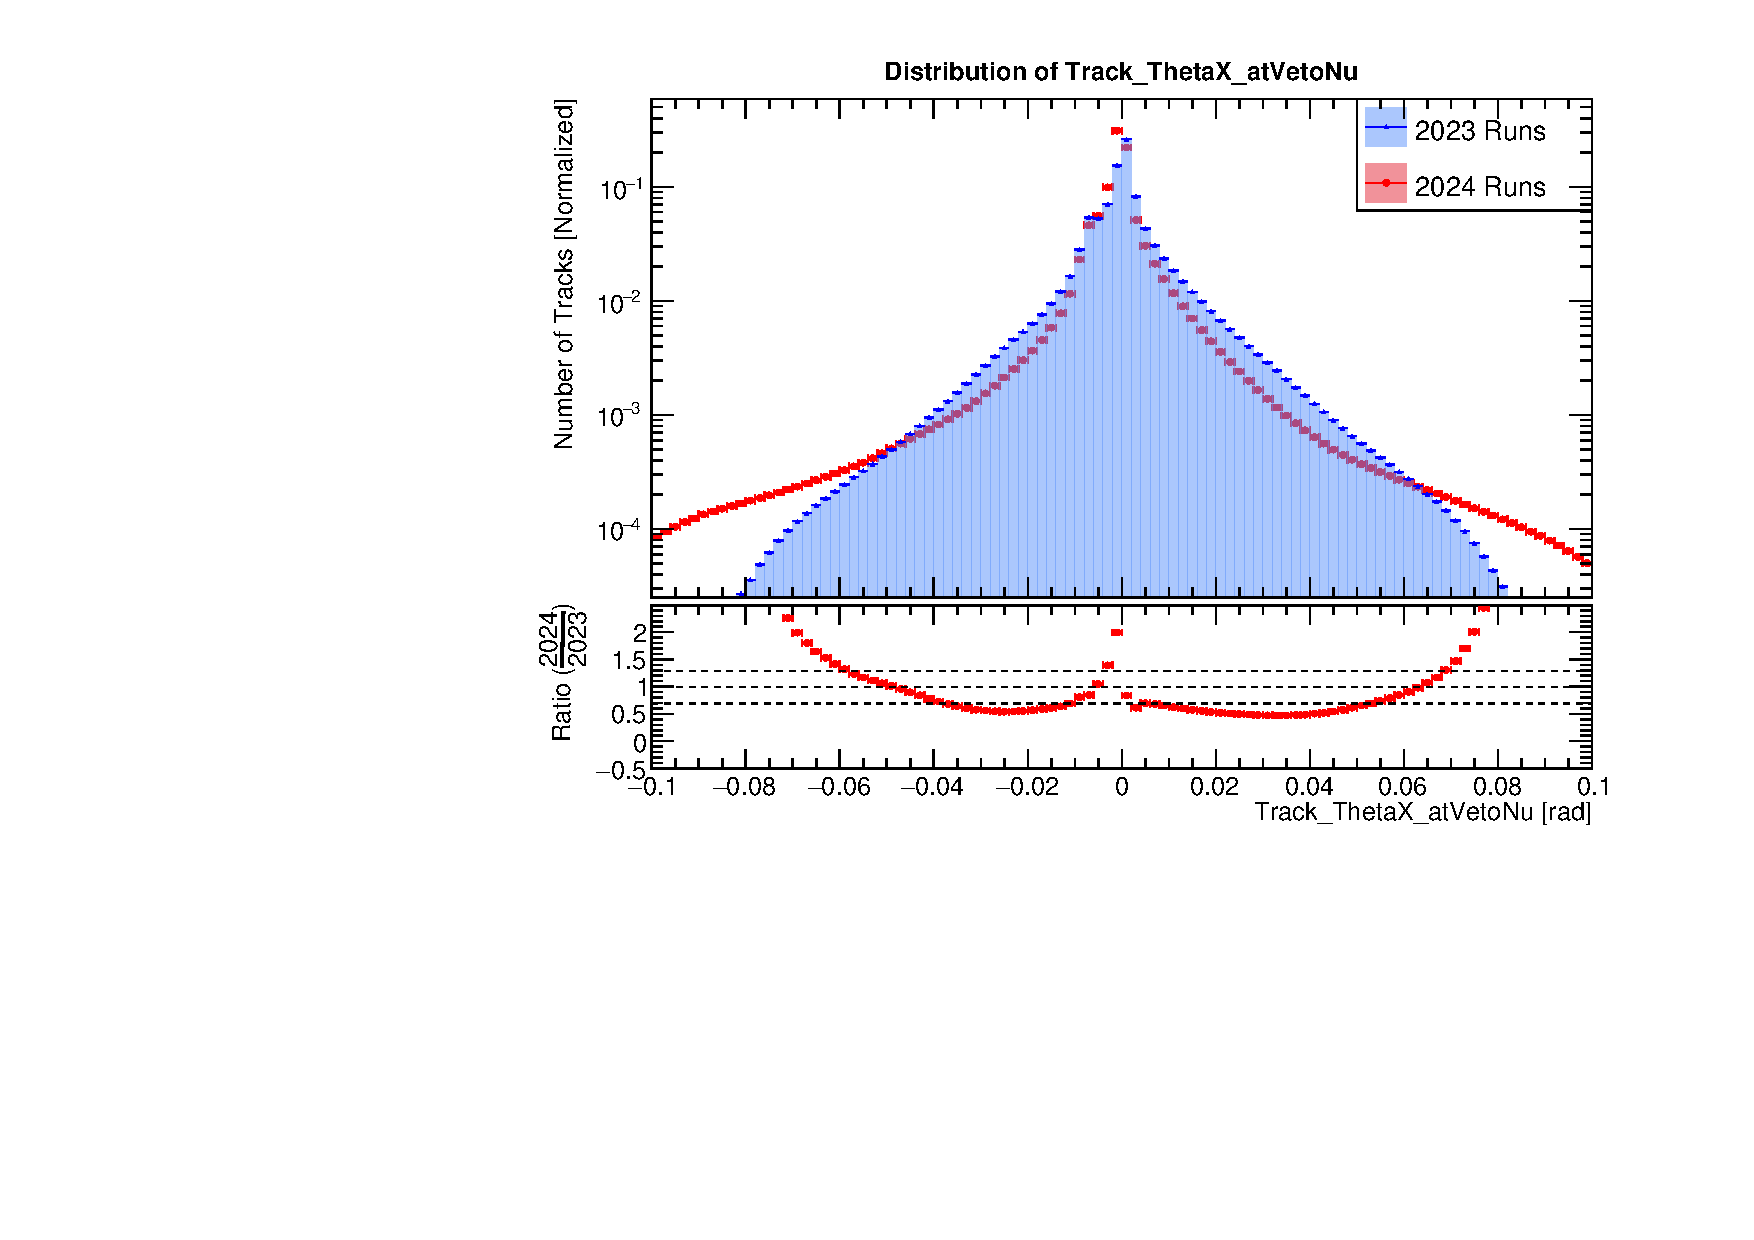
\includegraphics[width=\linewidth] {\plots/Track_ThetaX_atVetoNu.pdf}
				\caption{Track ThetaX at VetoNu}
			\end{figure}
		\end{column}
		\begin{column}{0.5\textwidth}
			\begin{figure}
				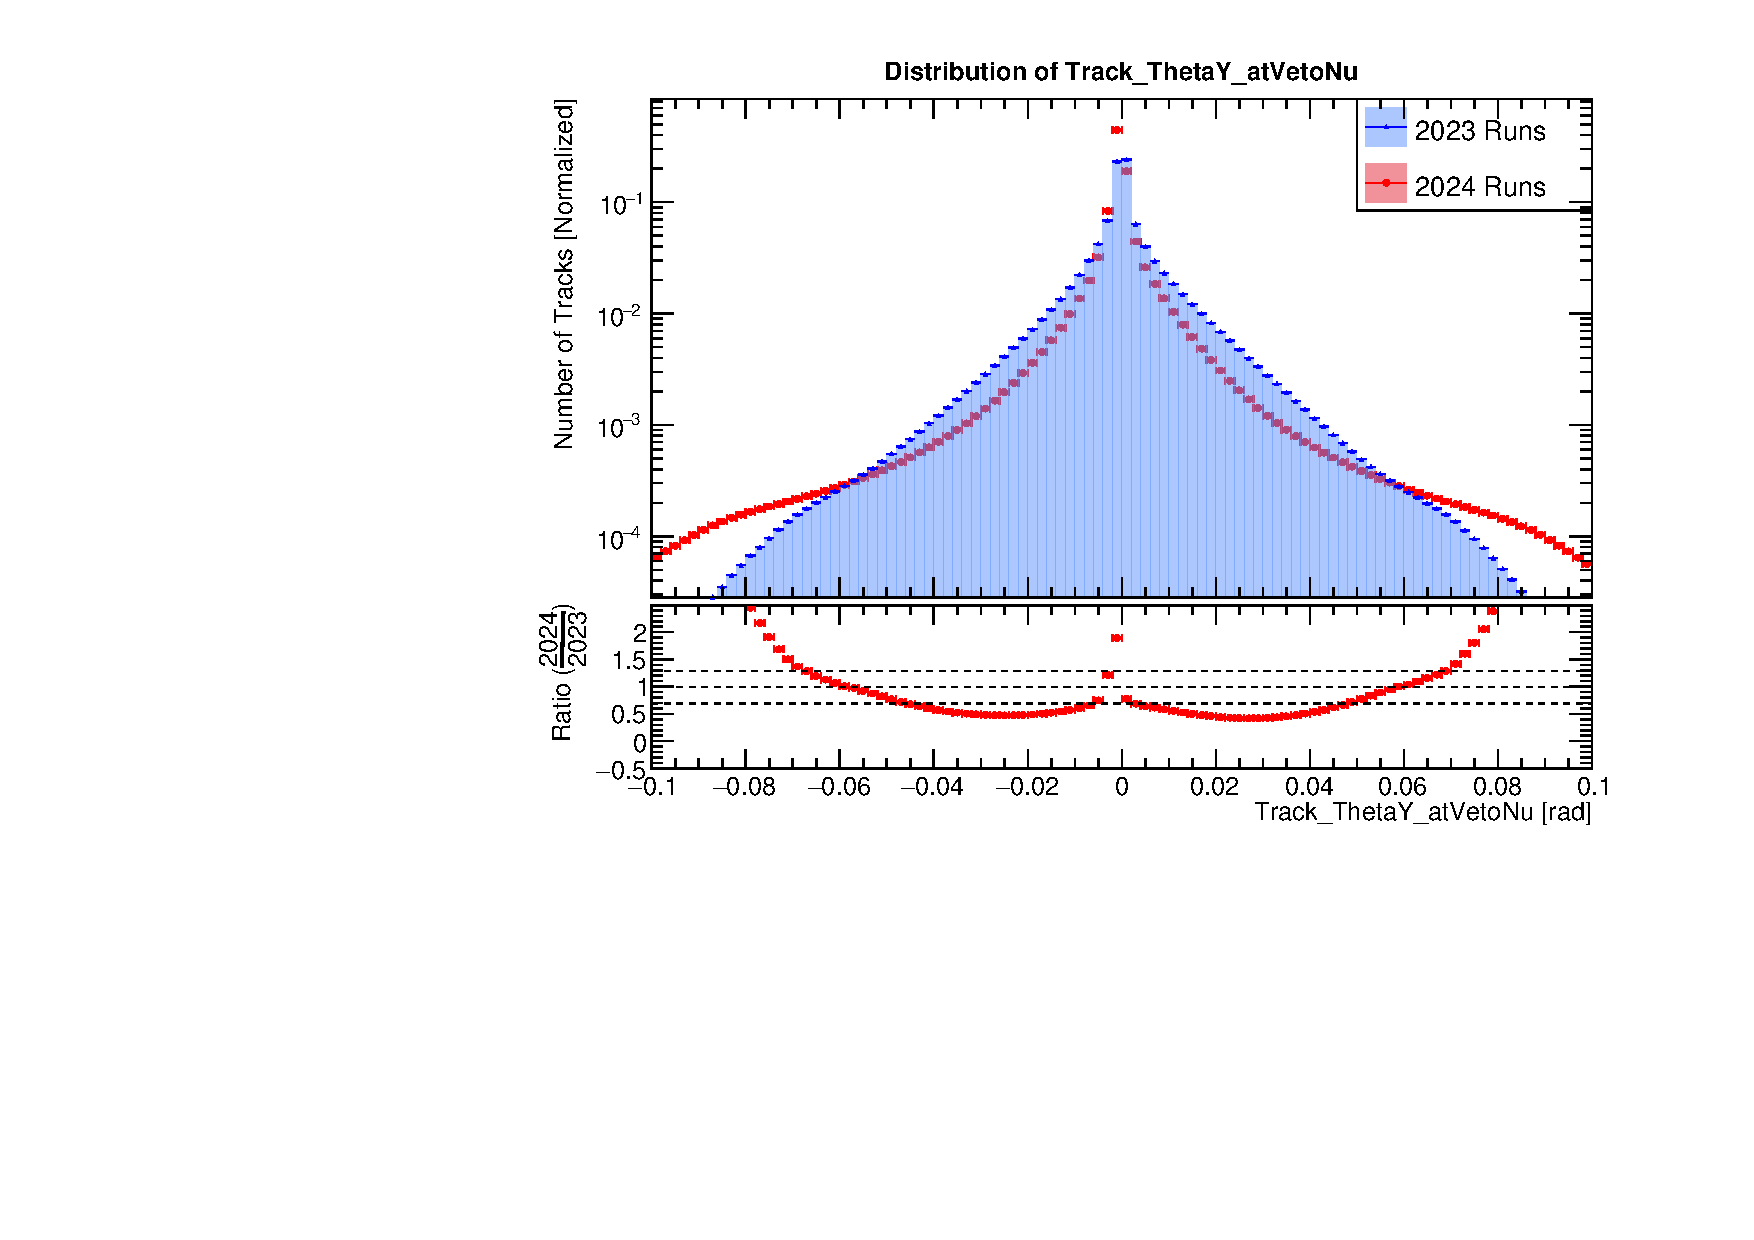
\includegraphics[width=\linewidth] {\plots/Track_ThetaY_atVetoNu.pdf}
				\caption{Track ThetaY at VetoNu}
			\end{figure}
		\end{column}
	\end{columns}
	\begin{itemize}
		\item Needs investigation to understand why the difference
	\end{itemize}
\end{frame}

\begin{subframe}{Track Momenta at VetoStation 1 [SKIP]}
	\begin{columns}
		\begin{column}{0.5\textwidth}
			\begin{figure}
				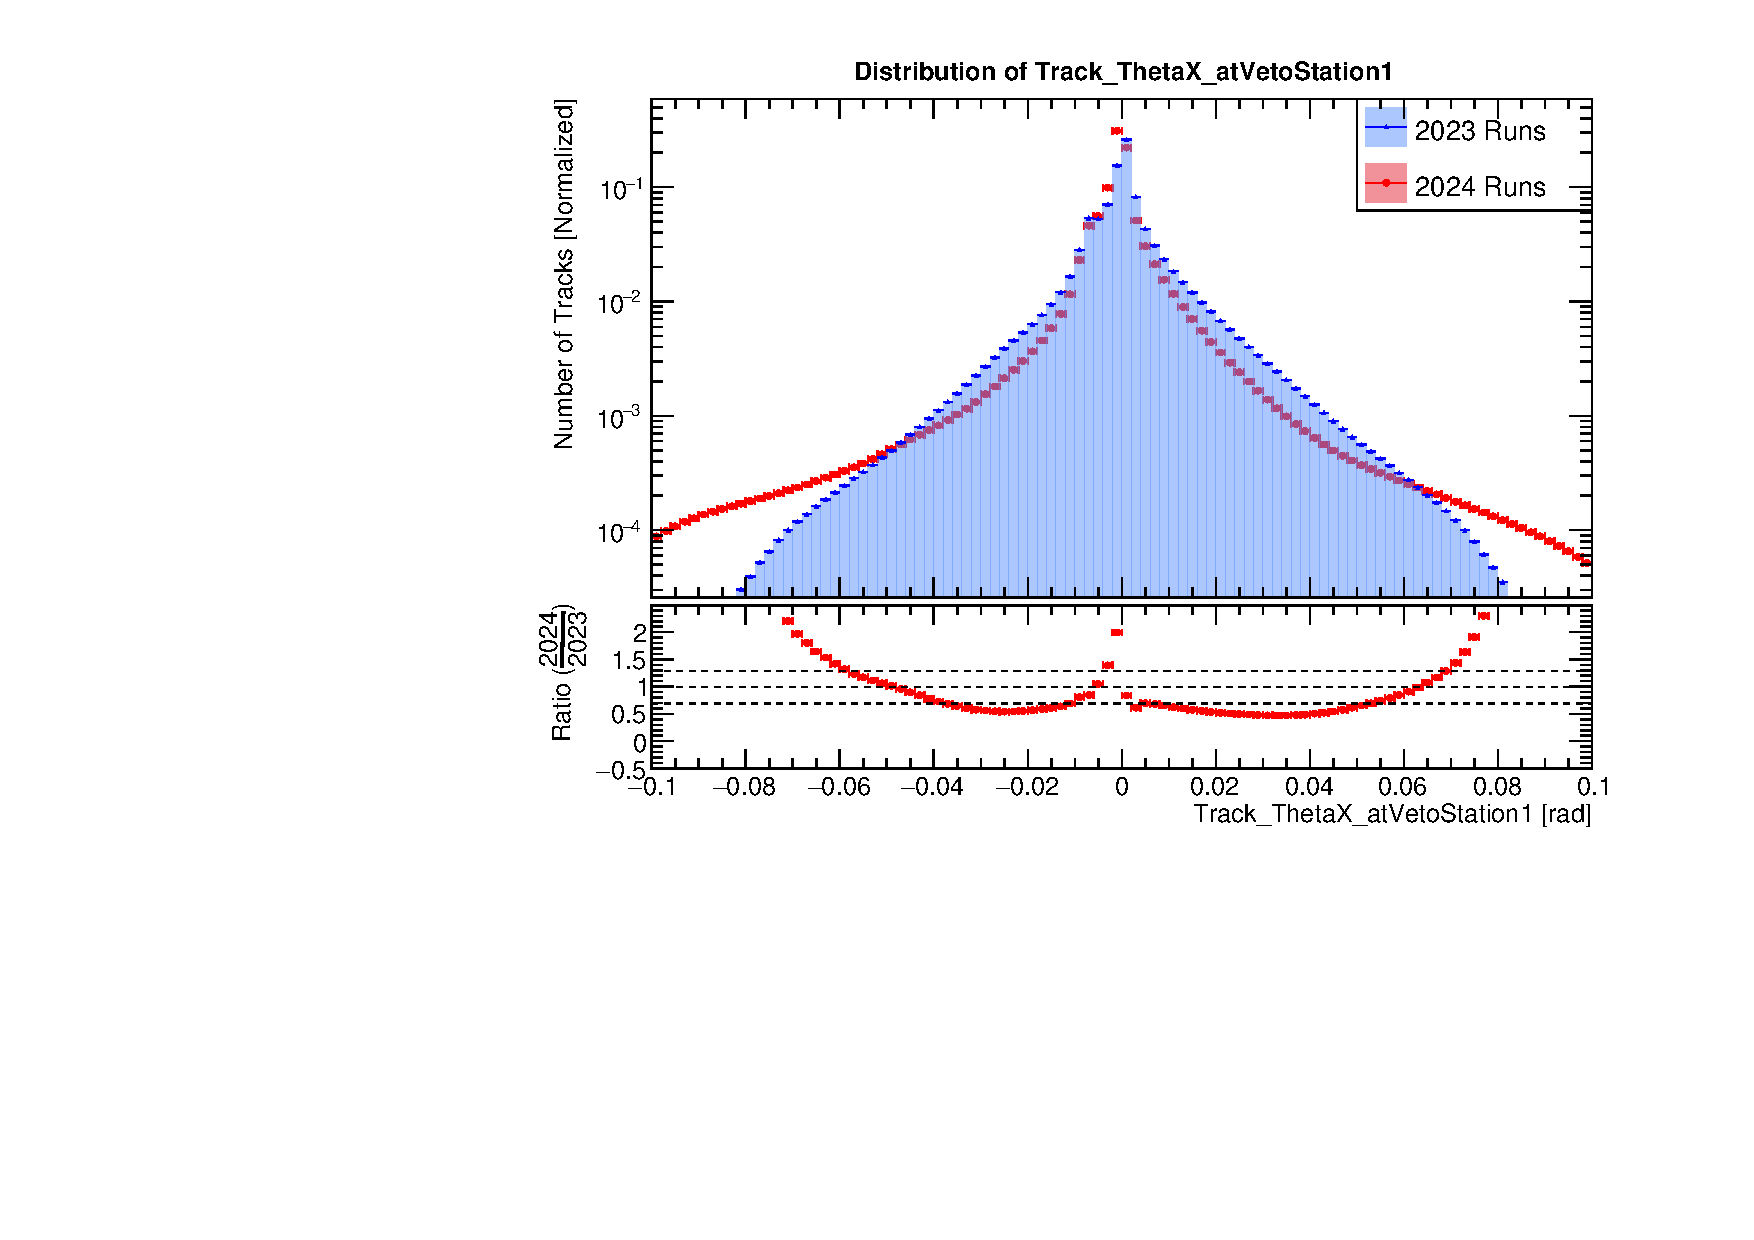
\includegraphics[width=\linewidth] {\plots/Track_ThetaX_atVetoStation1.pdf}
				\caption{Track ThetaX at atVetoStation 1}
			\end{figure}
		\end{column}
		\begin{column}{0.5\textwidth}
			\begin{figure}
				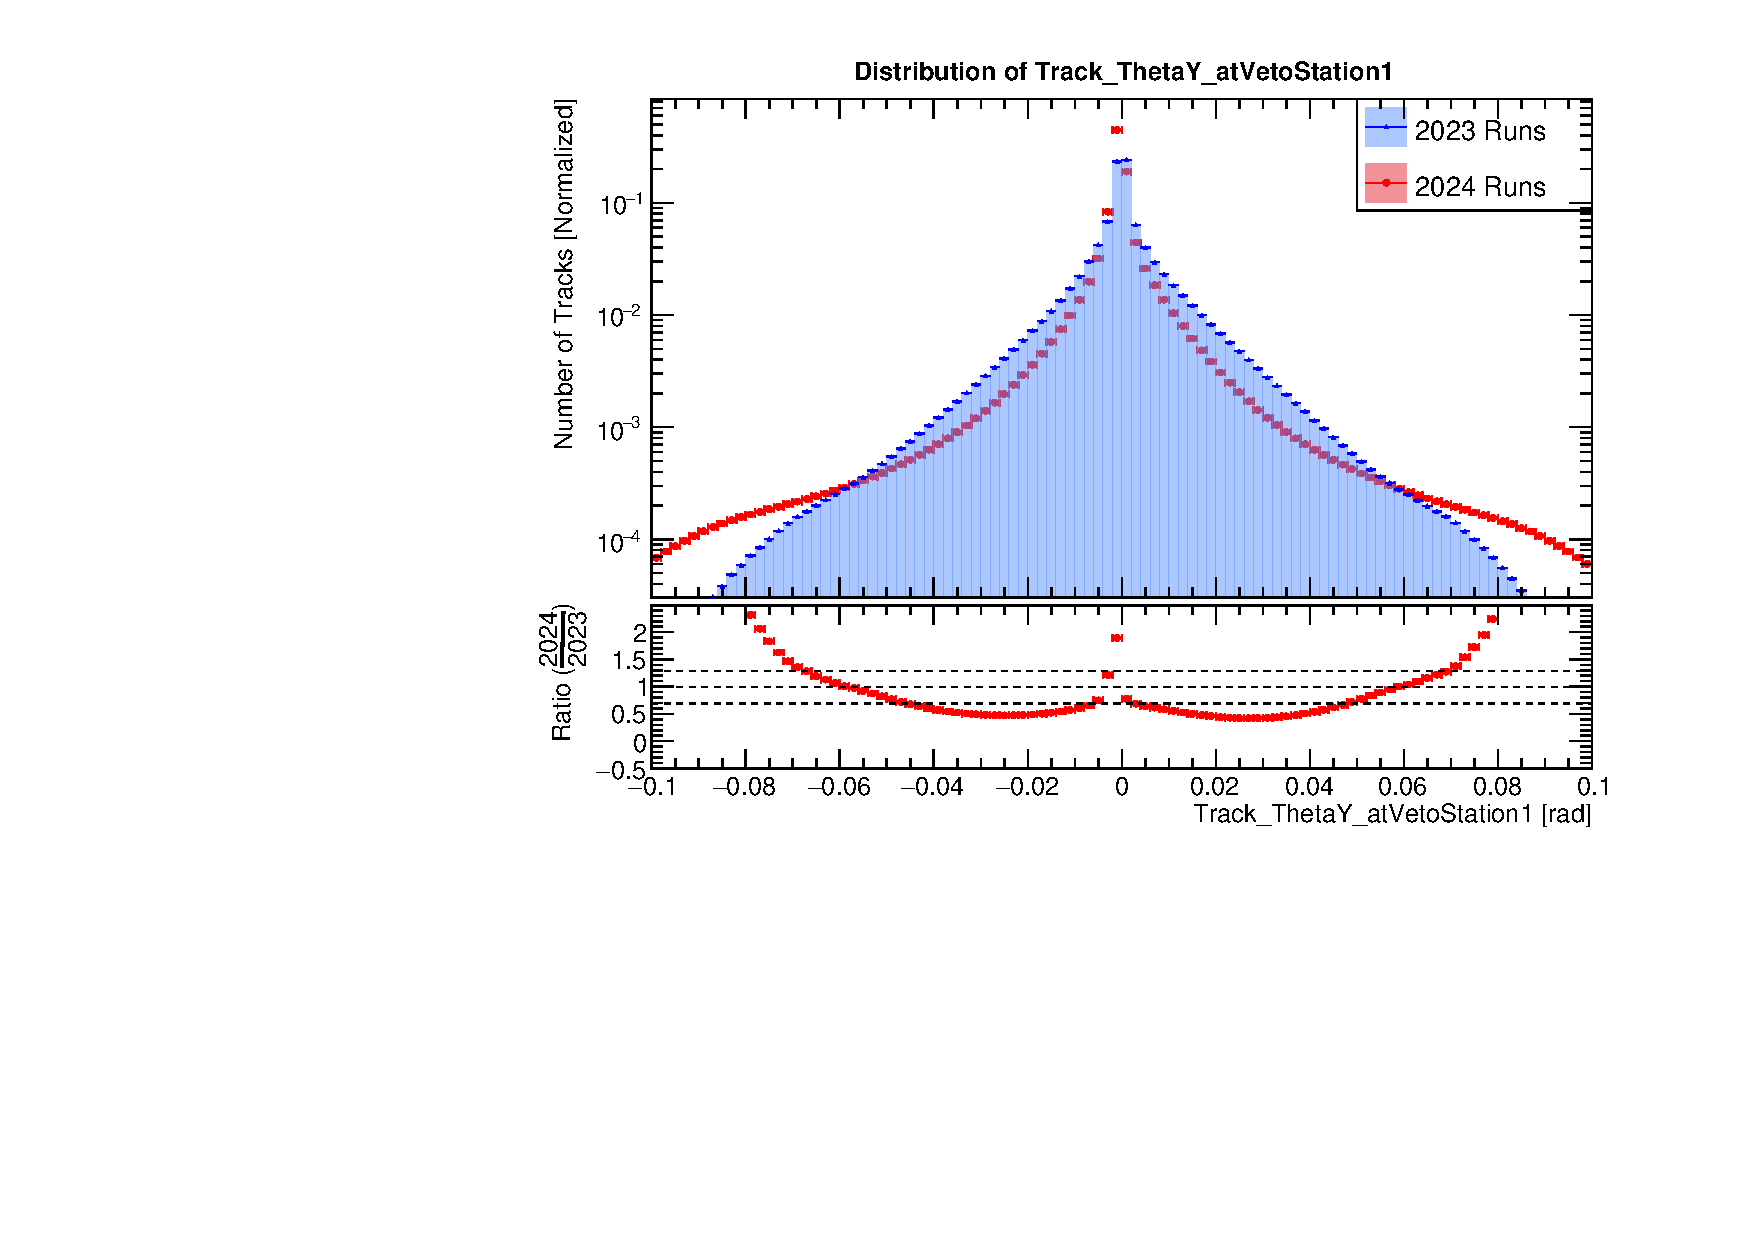
\includegraphics[width=\linewidth] {\plots/Track_ThetaY_atVetoStation1.pdf}
				\caption{Track ThetaY at VetoStation 1}
			\end{figure}
		\end{column}
	\end{columns}
\end{subframe}

\begin{subframe}{Track Momenta at VetoStation 2 [SKIP]}
	\begin{columns}
		\begin{column}{0.5\textwidth}
			\begin{figure}
				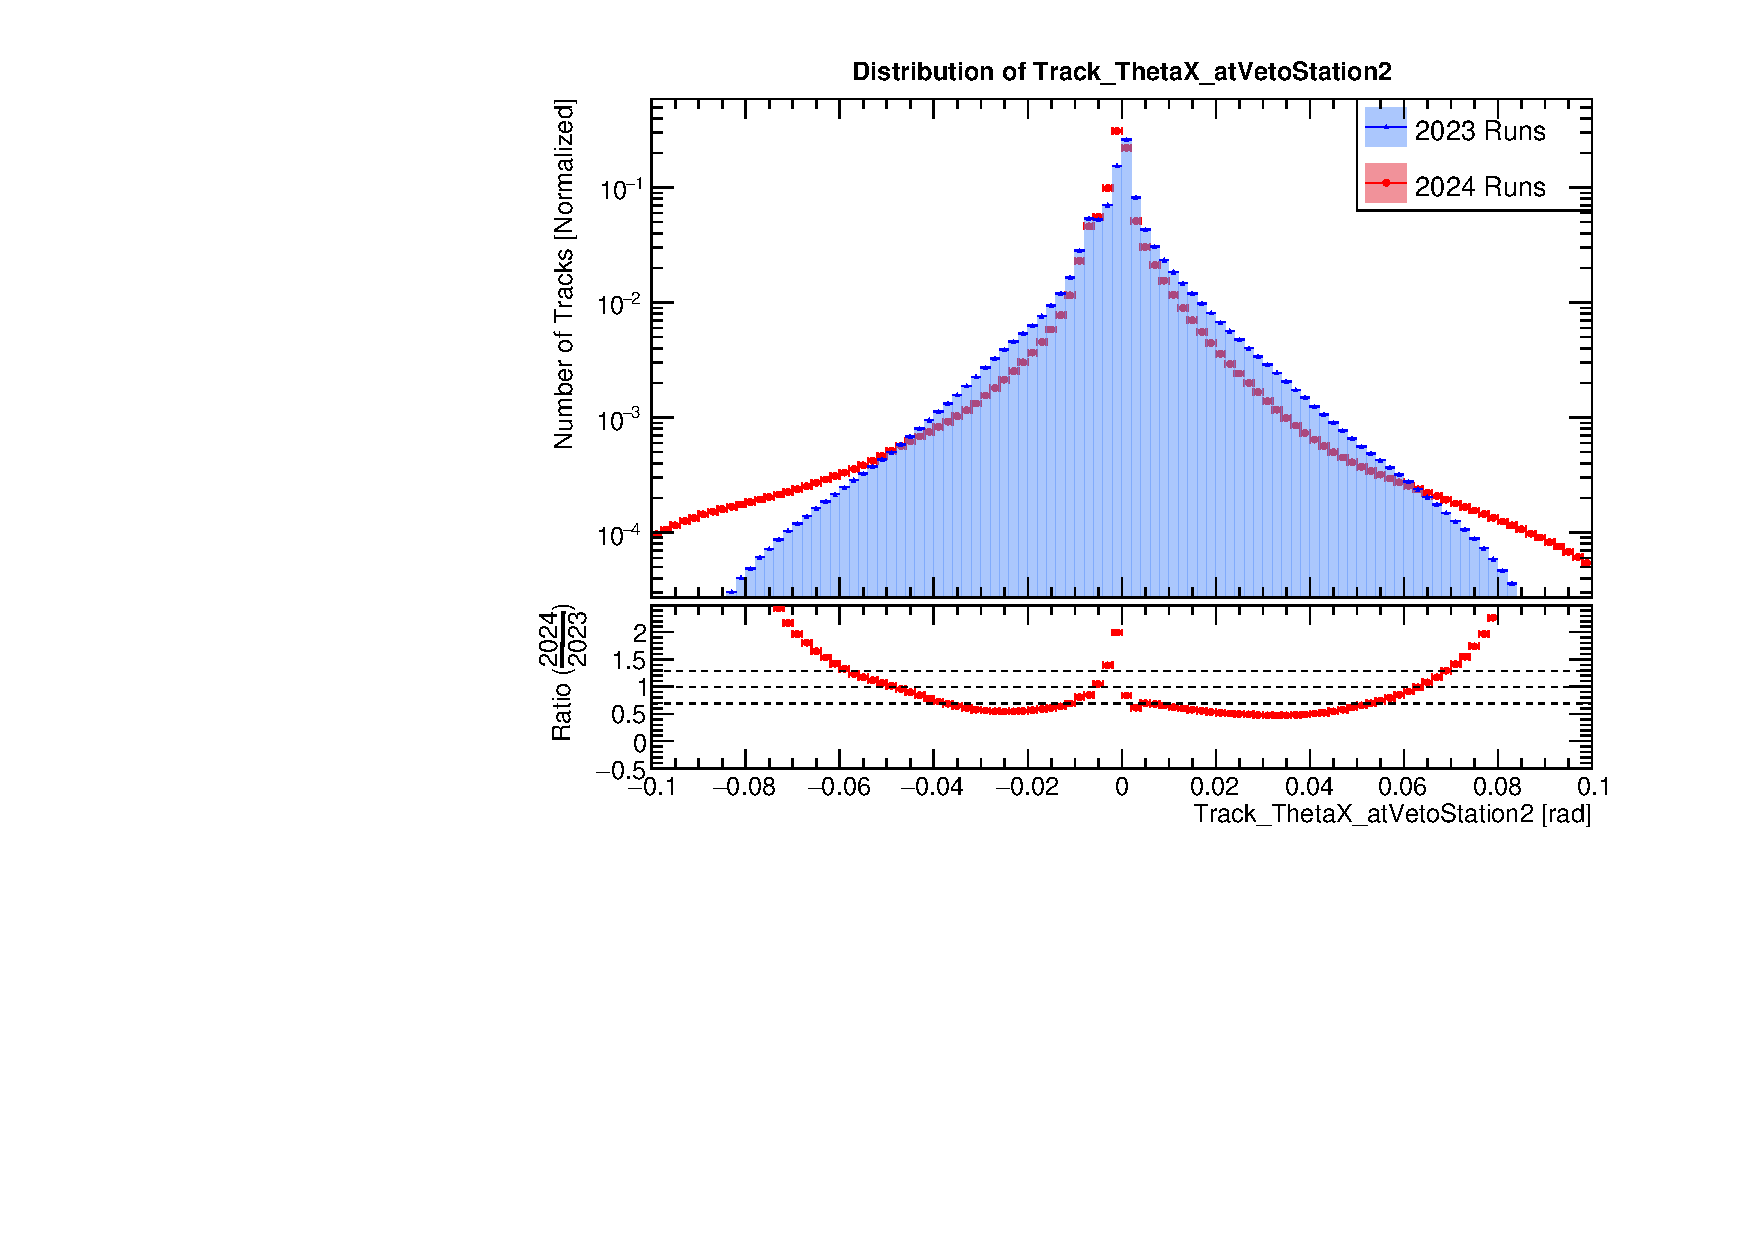
\includegraphics[width=\linewidth] {\plots/Track_ThetaX_atVetoStation2.pdf}
				\caption{Track ThetaX at VetoStation 2}
			\end{figure}
		\end{column}
		\begin{column}{0.5\textwidth}
			\begin{figure}
				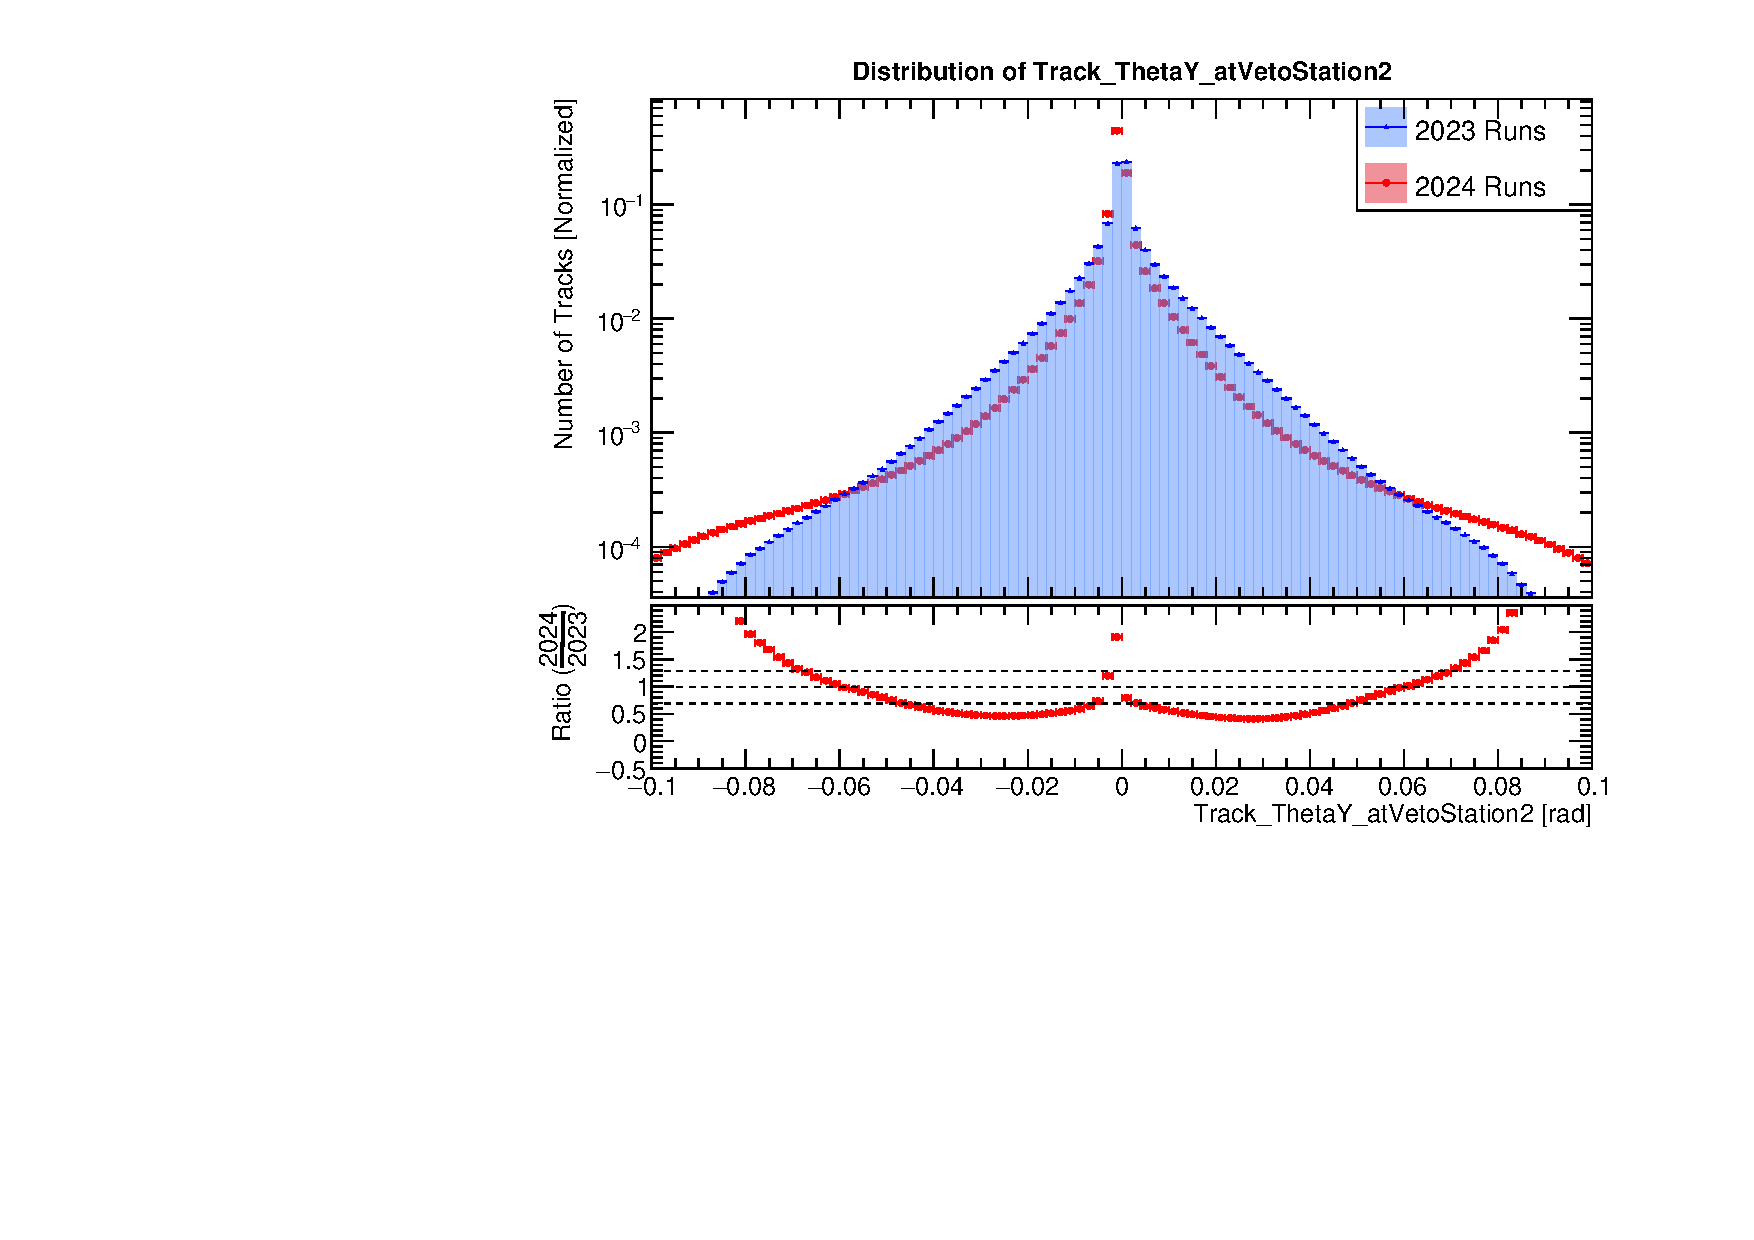
\includegraphics[width=\linewidth] {\plots/Track_ThetaY_atVetoStation2.pdf}
				\caption{Track ThetaY at VetoStation 1}
			\end{figure}
		\end{column}
	\end{columns}
\end{subframe}

\begin{subframe}{Track Momenta at Trigger [SKIP]}
	\begin{columns}
		\begin{column}{0.5\textwidth}
			\begin{figure}
				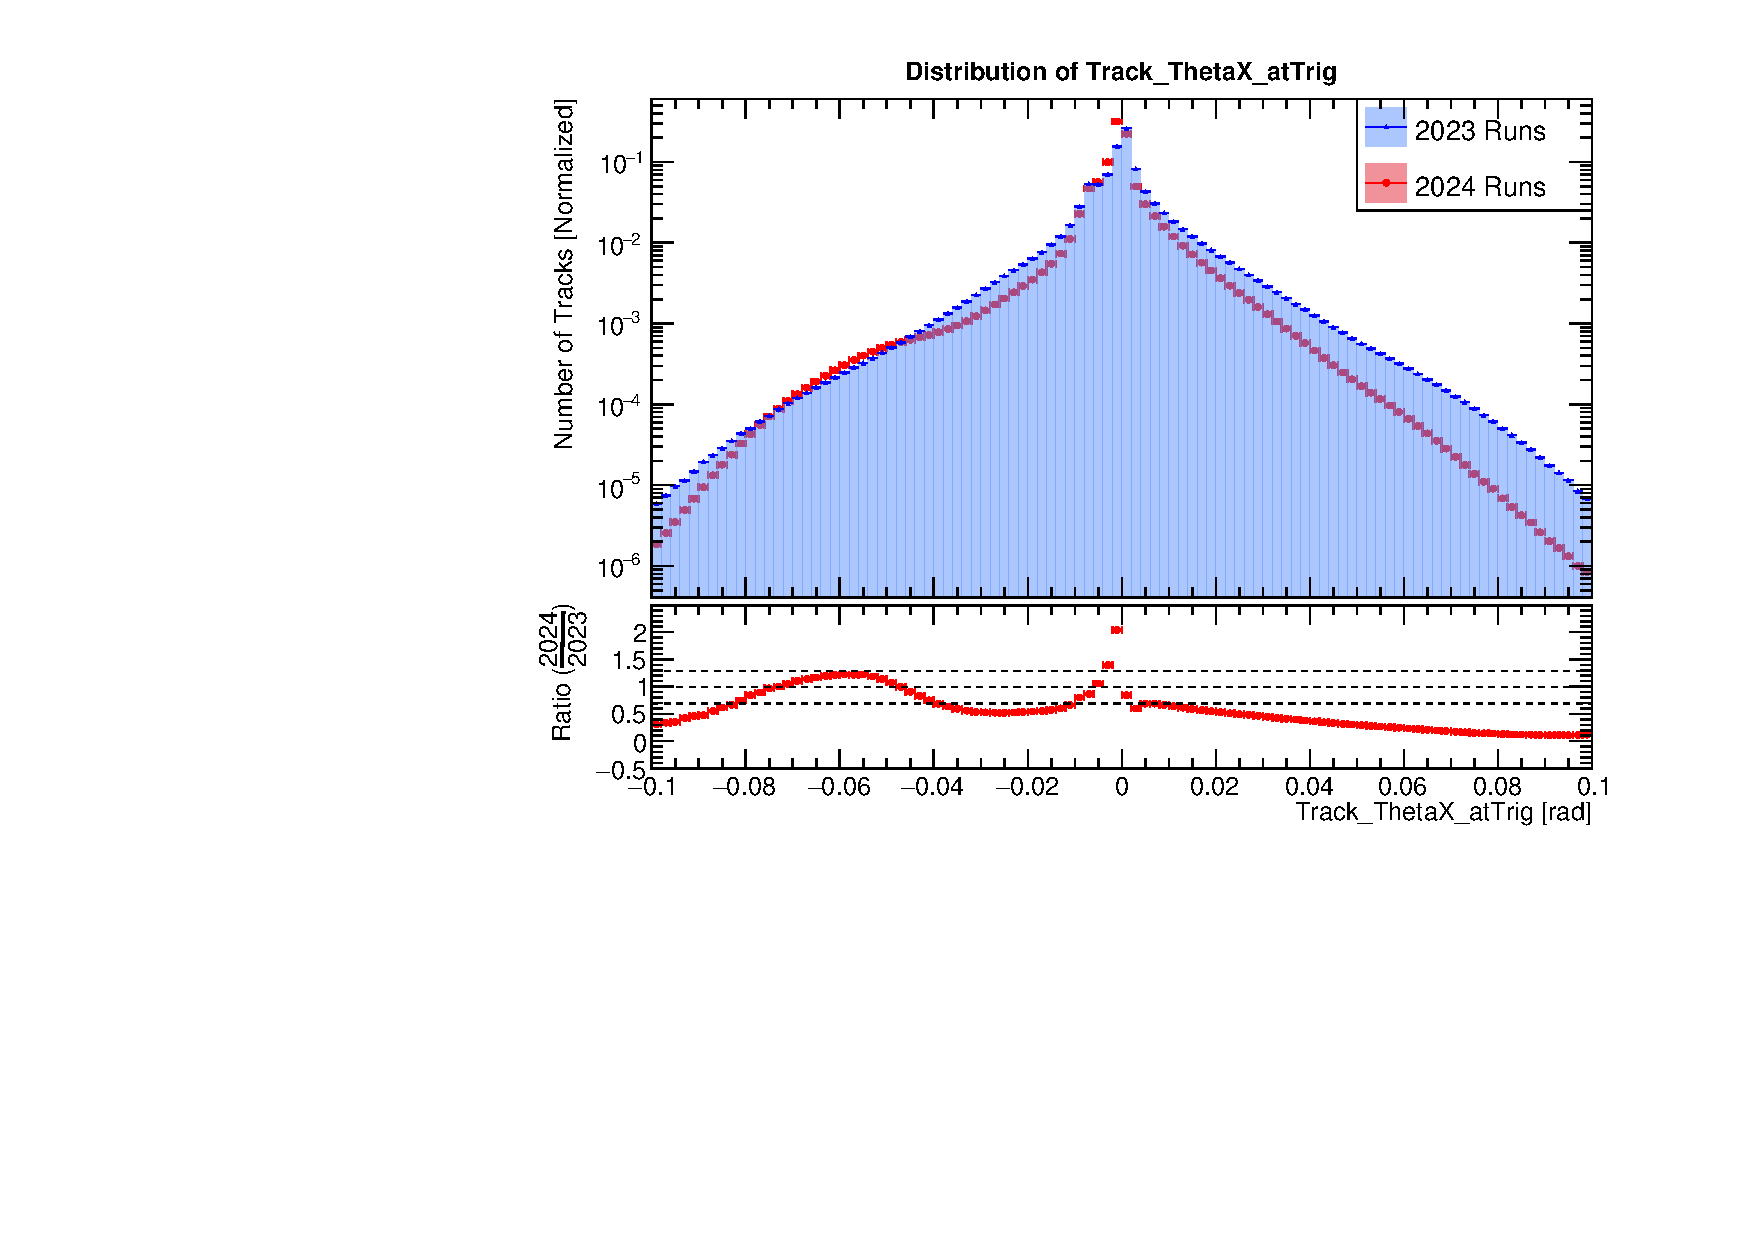
\includegraphics[width=\linewidth] {\plots/Track_ThetaX_atTrig.pdf}
				\caption{Track ThetaX at Trigger}
			\end{figure}
		\end{column}
		\begin{column}{0.5\textwidth}
			\begin{figure}
				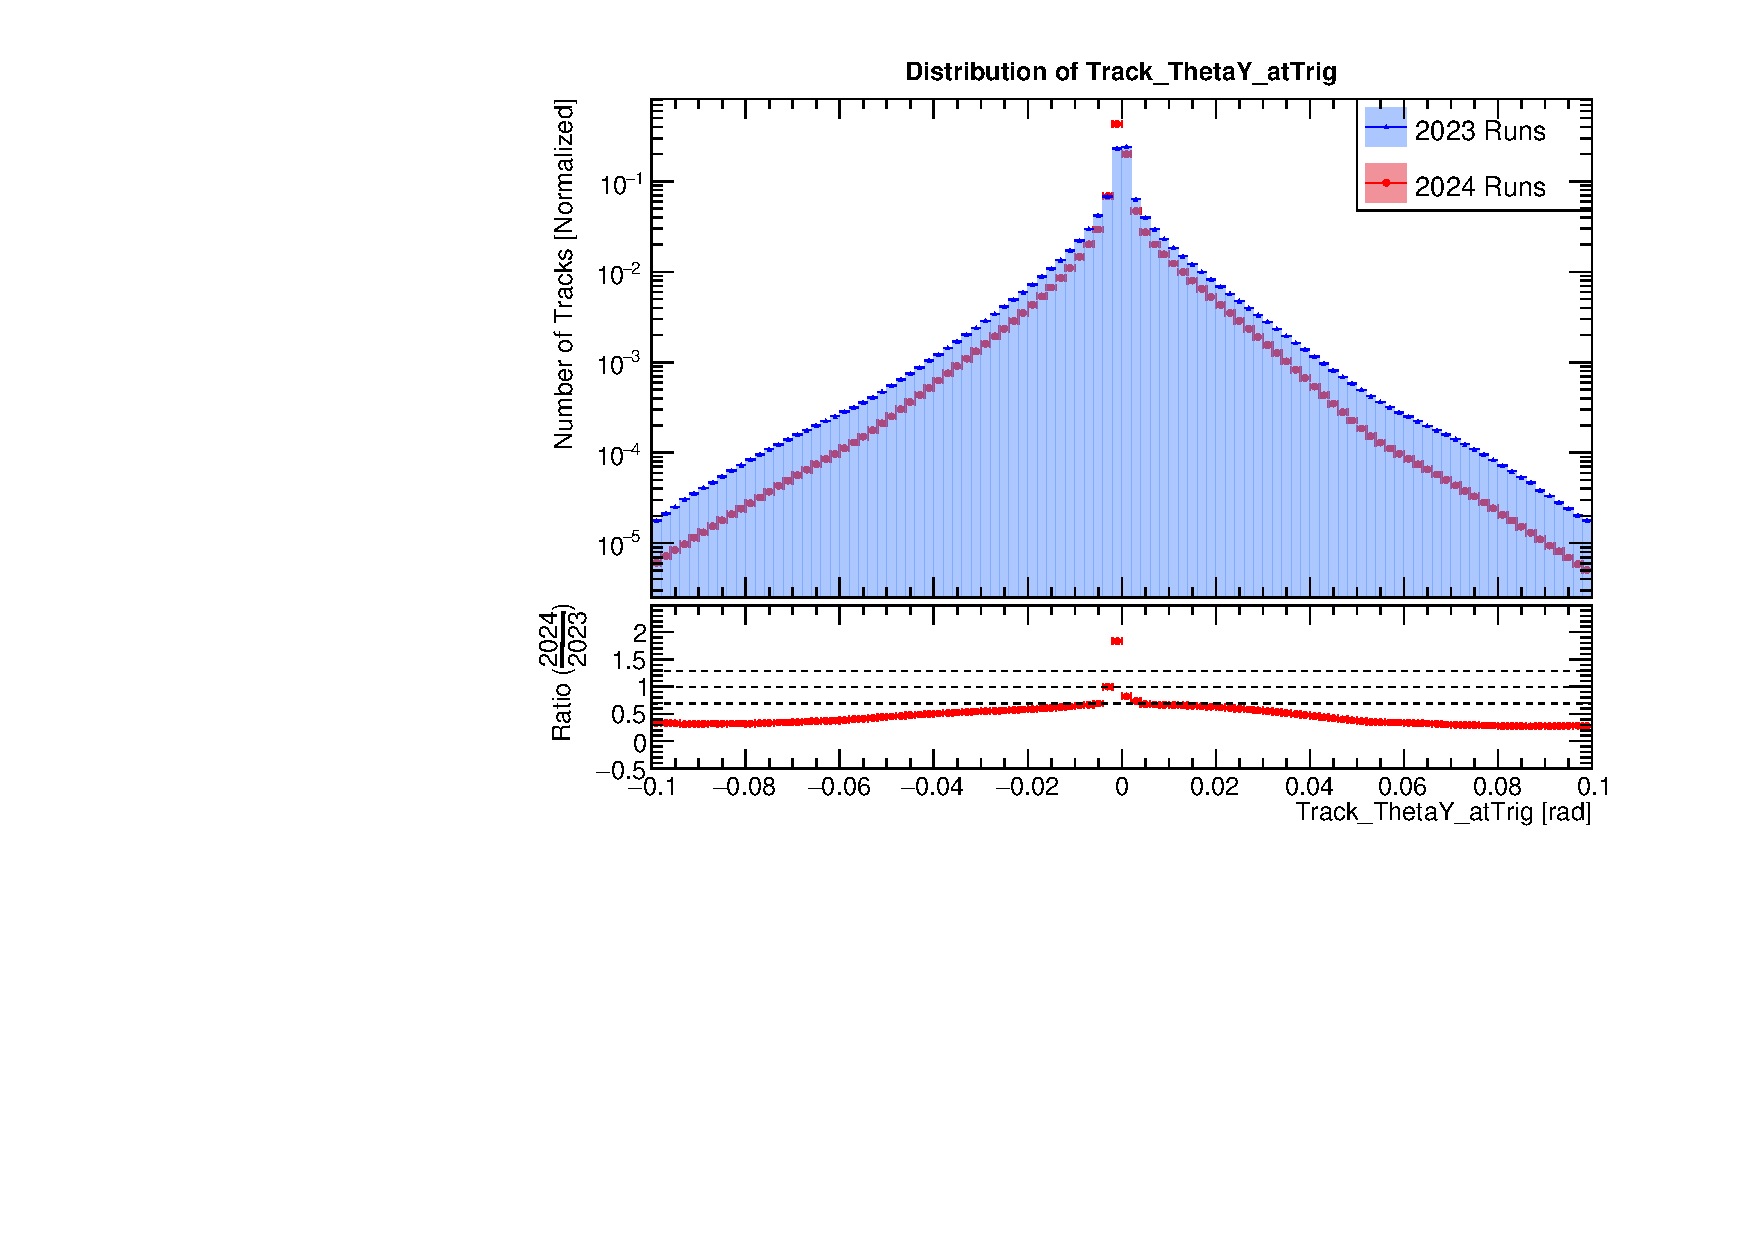
\includegraphics[width=\linewidth] {\plots/Track_ThetaY_atTrig.pdf}
				\caption{Track ThetaY at Trigger}
			\end{figure}
		\end{column}
	\end{columns}
\end{subframe}

\begin{frame}{Track Momenta at Tracking Station 1}
	\begin{columns}
		\begin{column}{0.5\textwidth}
			\begin{figure}
				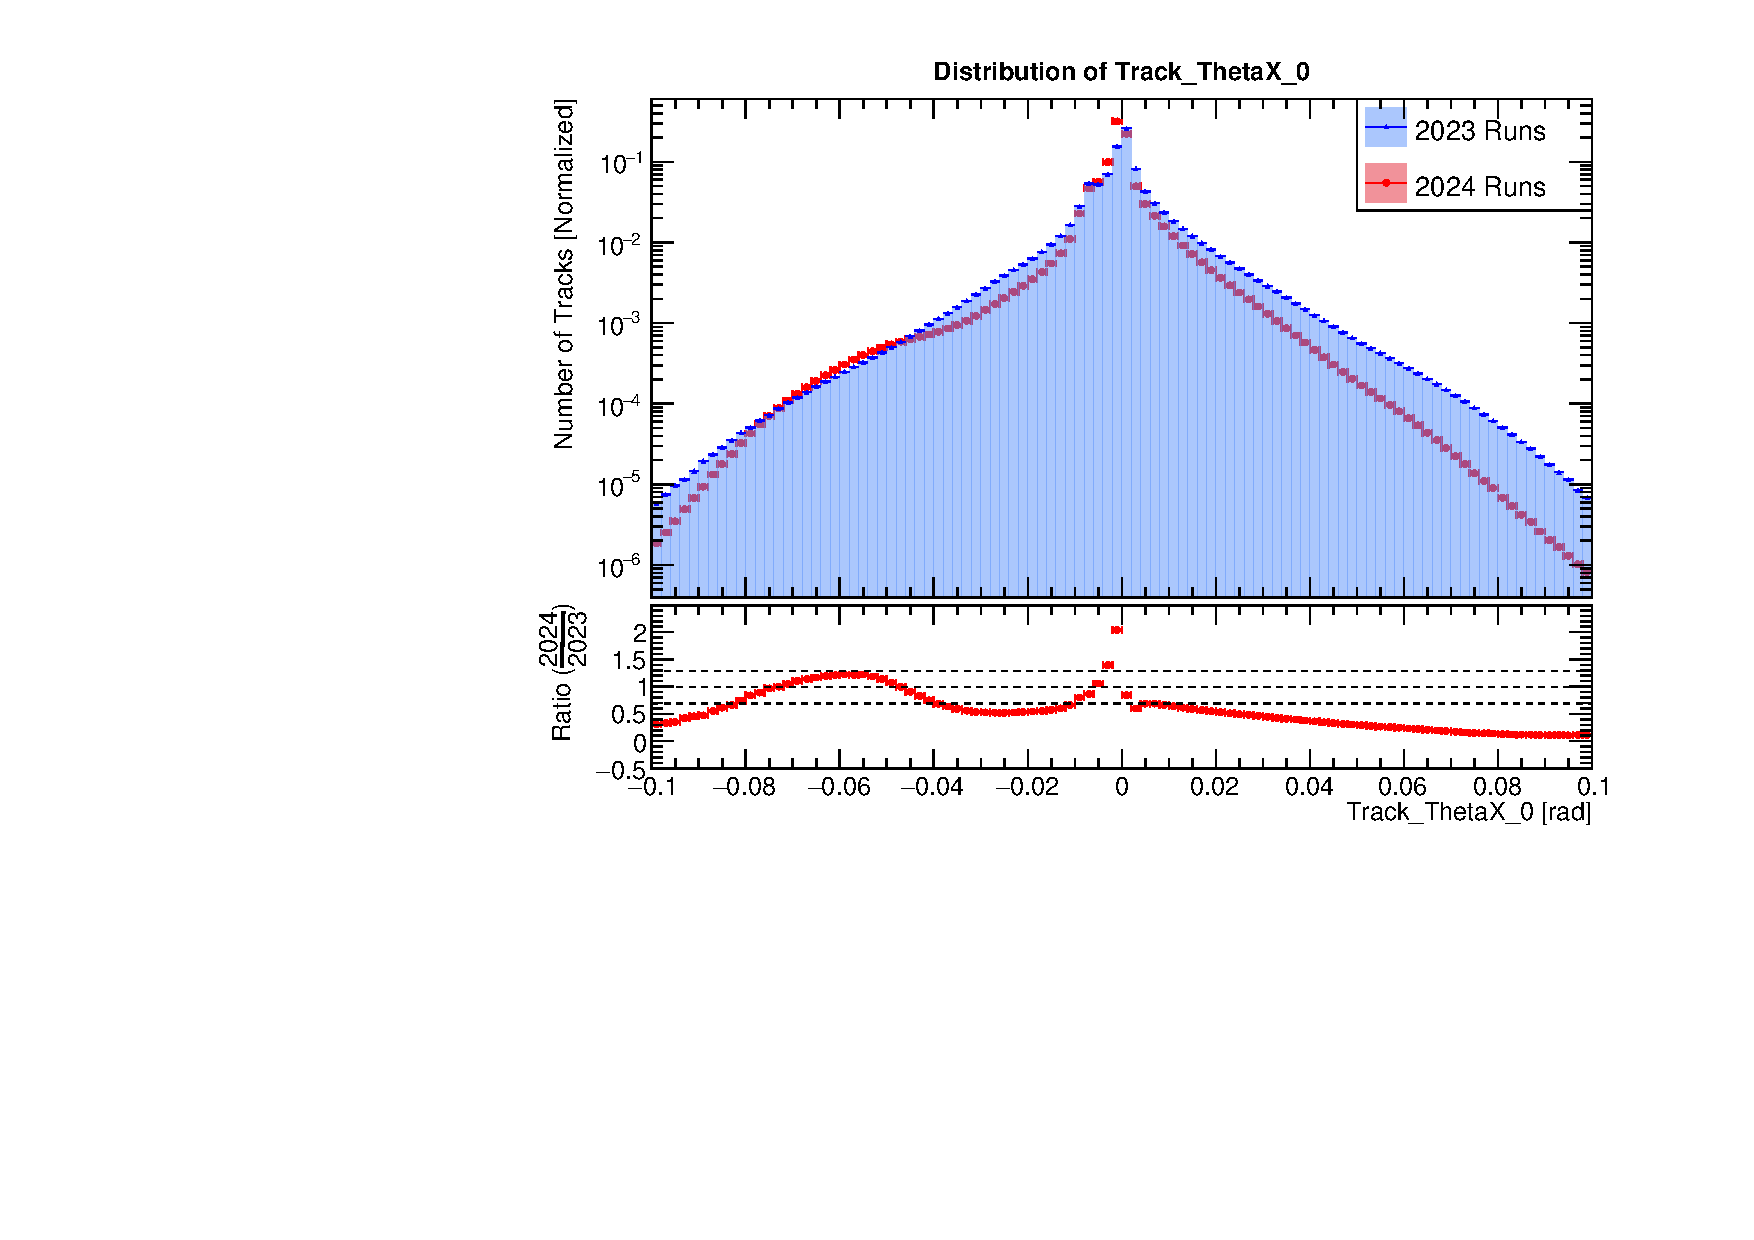
\includegraphics[width=\linewidth] {\plots/Track_ThetaX_0.pdf}
				\caption{Track ThetaX at Tracking Station 1}
			\end{figure}
		\end{column}
		\begin{column}{0.5\textwidth}
			\begin{figure}
				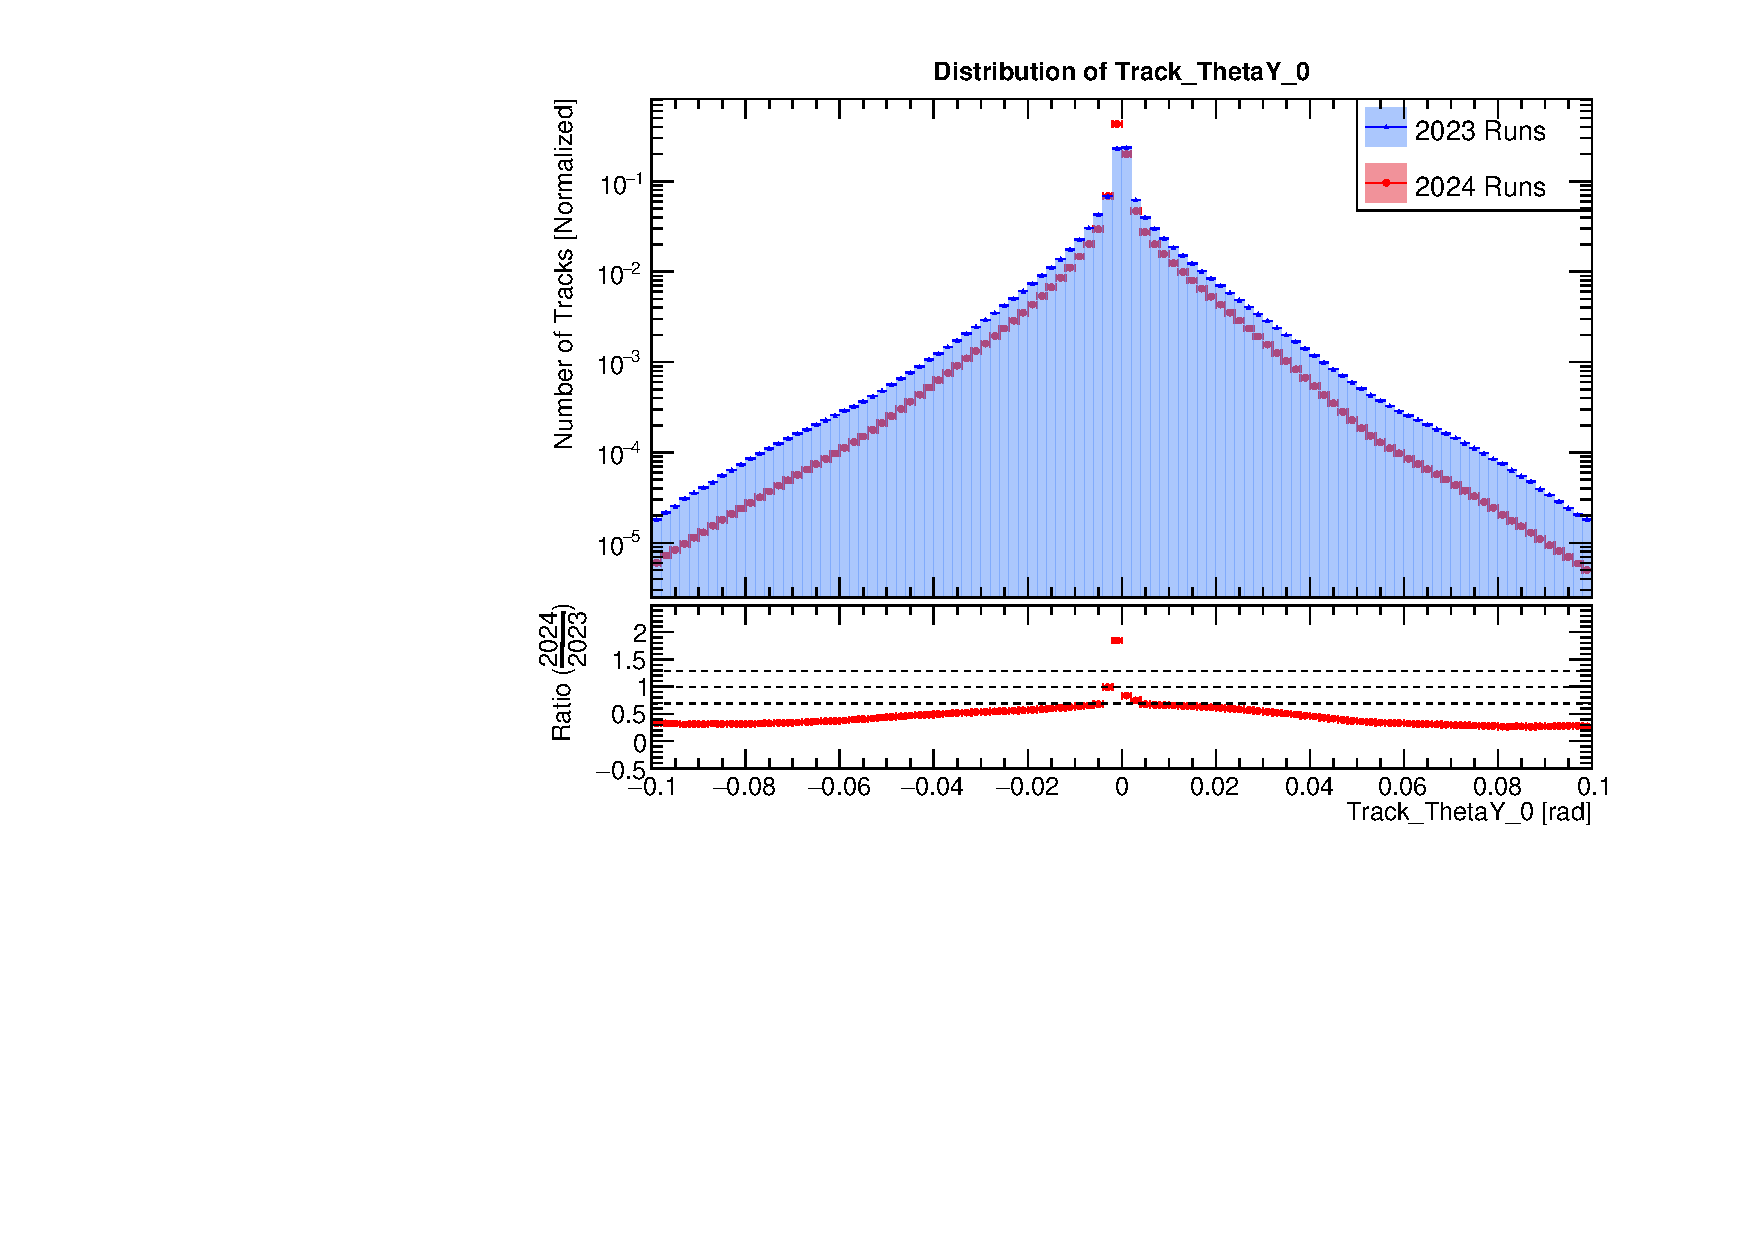
\includegraphics[width=\linewidth] {\plots/Track_ThetaY_0.pdf}
				\caption{Track ThetaY at Tracking Station 1}
			\end{figure}
		\end{column}
	\end{columns}
	\begin{itemize}
		\item There is a peak in 2024 data at -0.07 rad. Do we understand why?
		\item Similar features observed in the Background studies. [See \href{https://indico.cern.ch/event/1350790/contributions/5686387/attachments/2836819/4957405/Introduction.pdf}{Page 15-16}]
	\end{itemize}
\end{frame}

\begin{frame}{Track momentum at Tracking Station 3}
	\begin{columns}
		\begin{column}{0.5\textwidth}
			\begin{figure}
				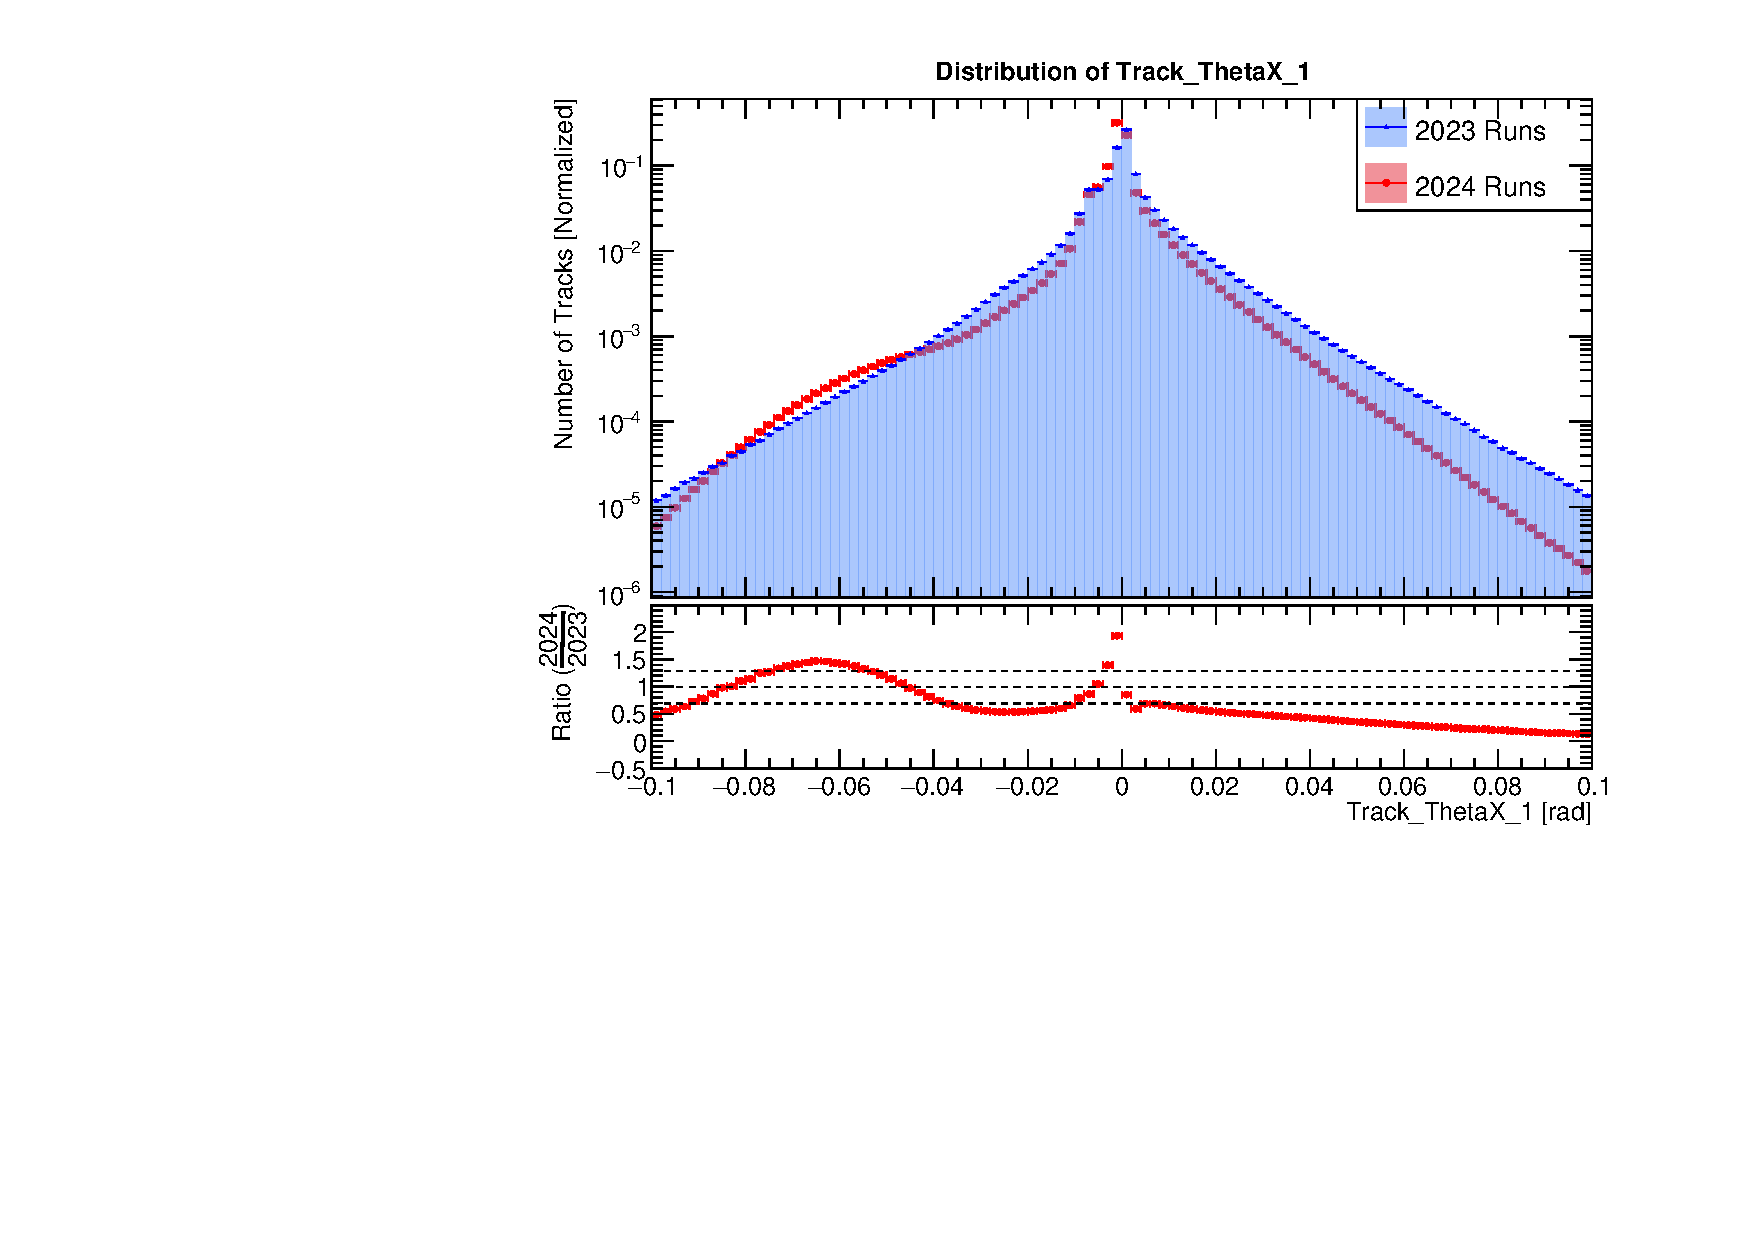
\includegraphics[width=\linewidth] {\plots/Track_ThetaX_1.pdf}
				\caption{Track ThetaX at Tracking Station 3}
			\end{figure}
		\end{column}
		\begin{column}{0.5\textwidth}
			\begin{figure}
				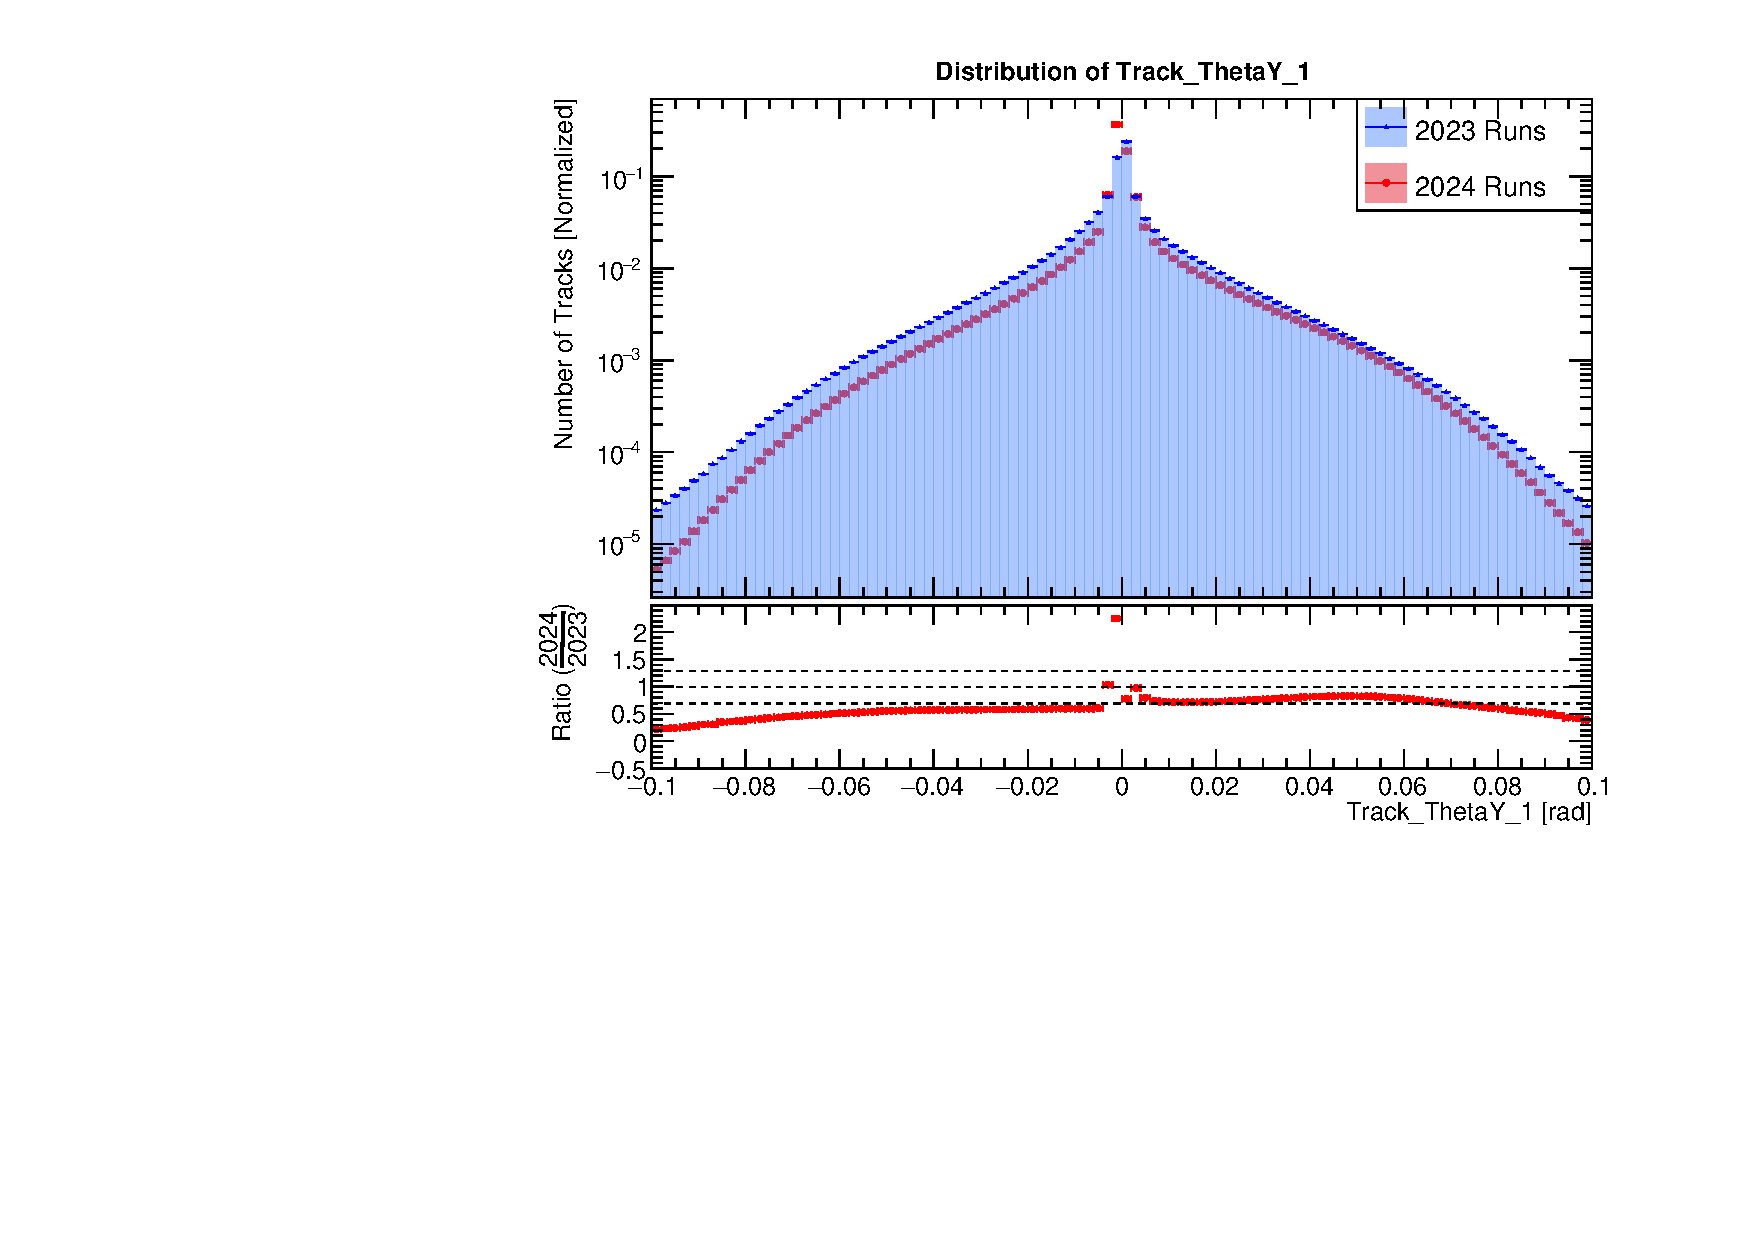
\includegraphics[width=\linewidth] {\plots/Track_ThetaY_1.pdf}
				\caption{Track ThetaX at Tracking Station 3}
			\end{figure}
		\end{column}
	\end{columns}
\end{frame}

\begin{subframe}{Track Momenta at Preshower 1 [SKIP]}
	\begin{columns}
		\begin{column}{0.5\textwidth}
			\begin{figure}
				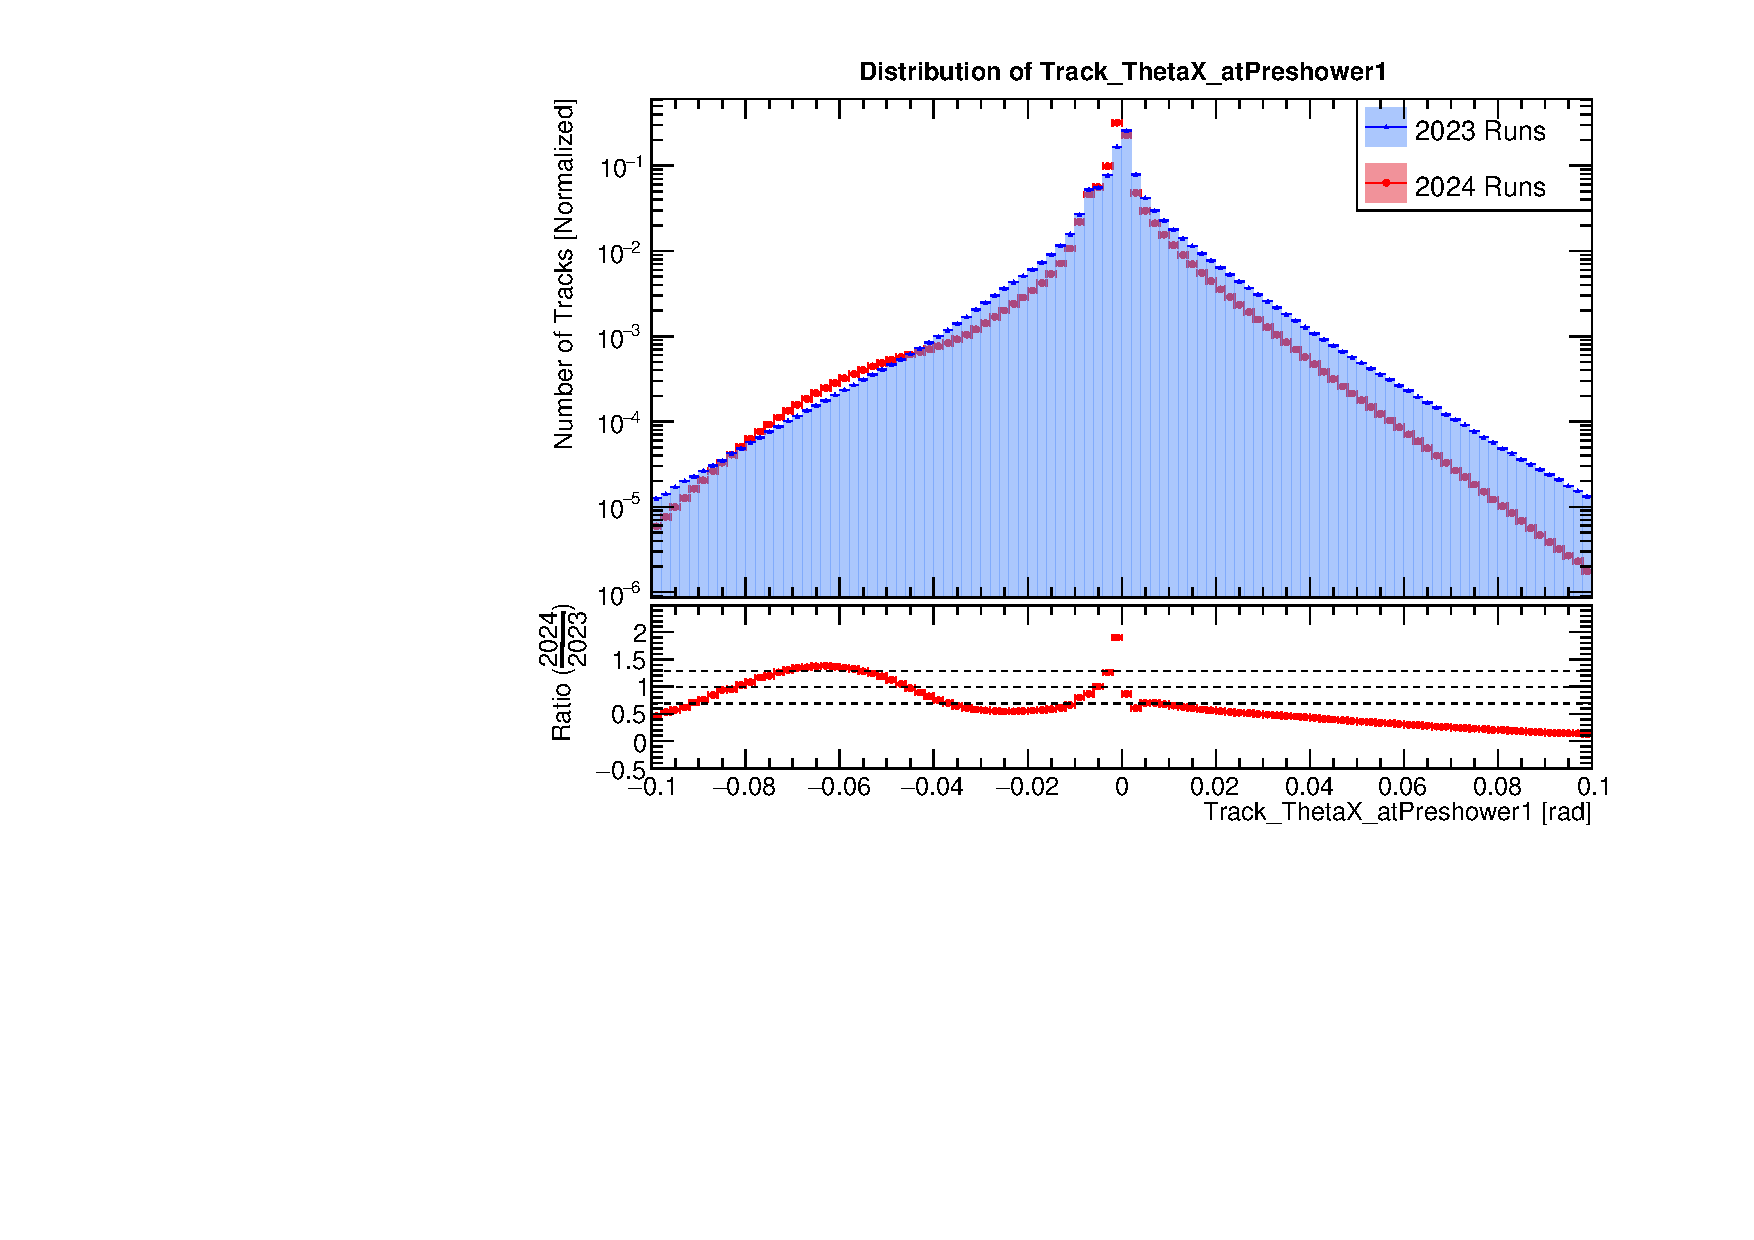
\includegraphics[width=\linewidth] {\plots/Track_ThetaX_atPreshower1.pdf}
				\caption{Track ThetaX at Preshower 1}
			\end{figure}
		\end{column}
		\begin{column}{0.5\textwidth}
			\begin{figure}
				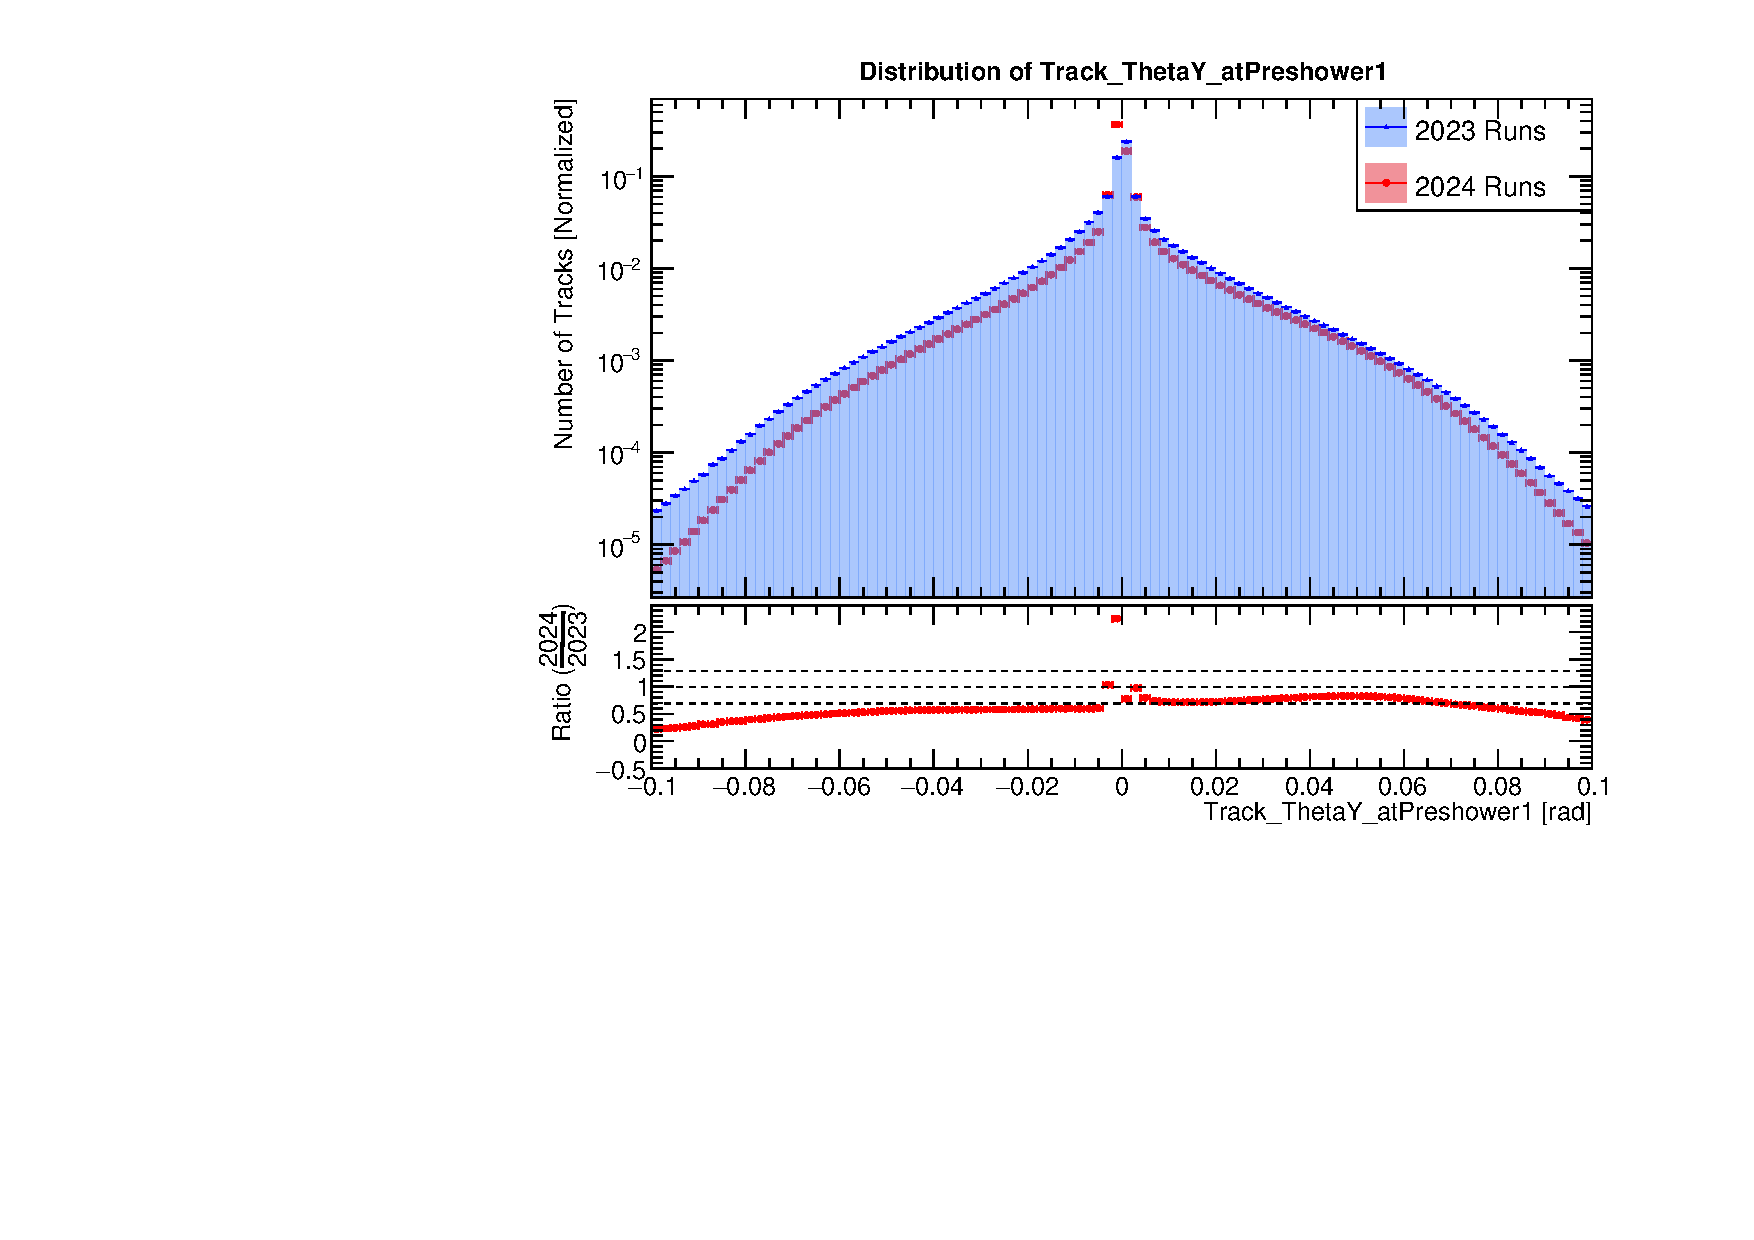
\includegraphics[width=\linewidth] {\plots/Track_ThetaY_atPreshower1.pdf}
				\caption{Track ThetaY at Preshower 1}
			\end{figure}
		\end{column}
	\end{columns}
\end{subframe}

\begin{subframe}{Track Momenta at Preshower 2 [SKIP]}
	\begin{columns}
		\begin{column}{0.5\textwidth}
			\begin{figure}
				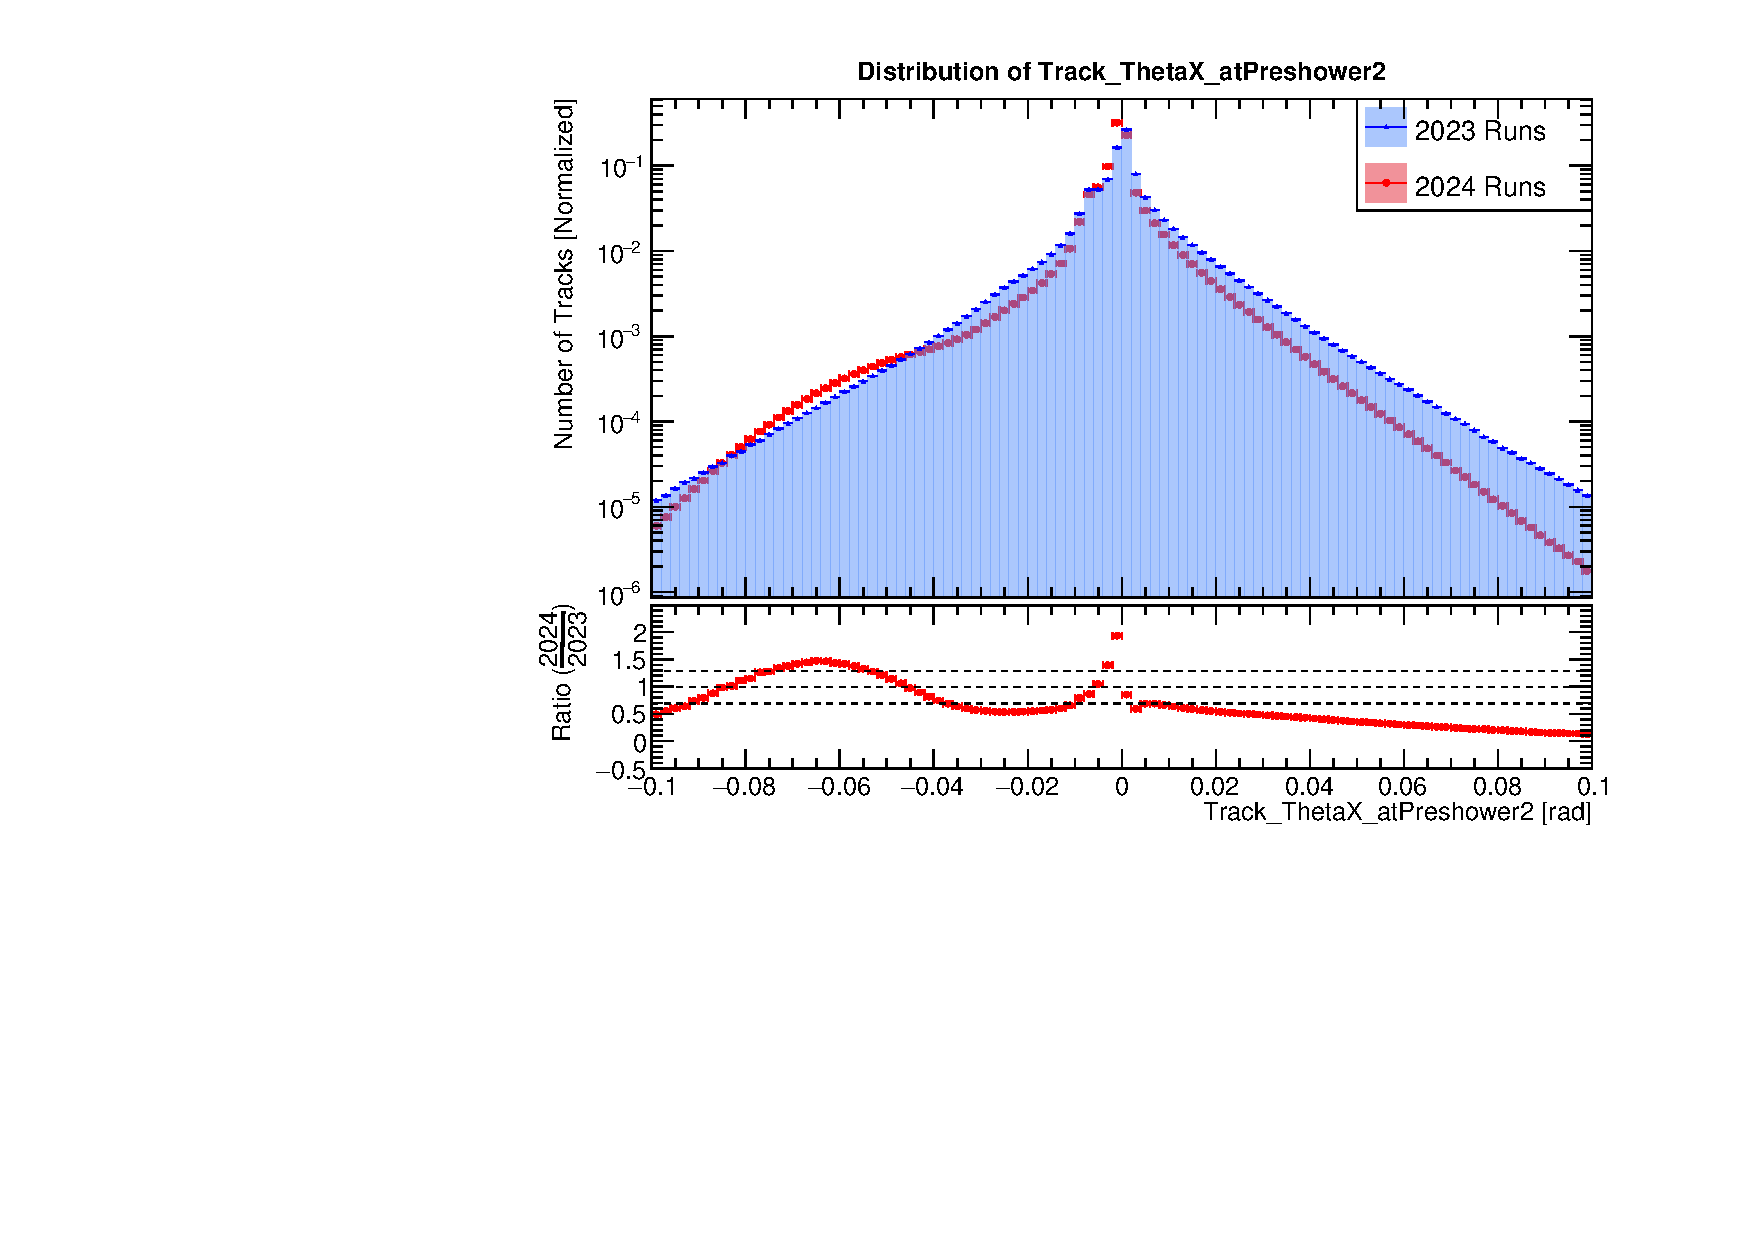
\includegraphics[width=\linewidth] {\plots/Track_ThetaX_atPreshower2.pdf}
				\caption{Track ThetaX at Preshower 2}
			\end{figure}
		\end{column}
		\begin{column}{0.5\textwidth}
			\begin{figure}
				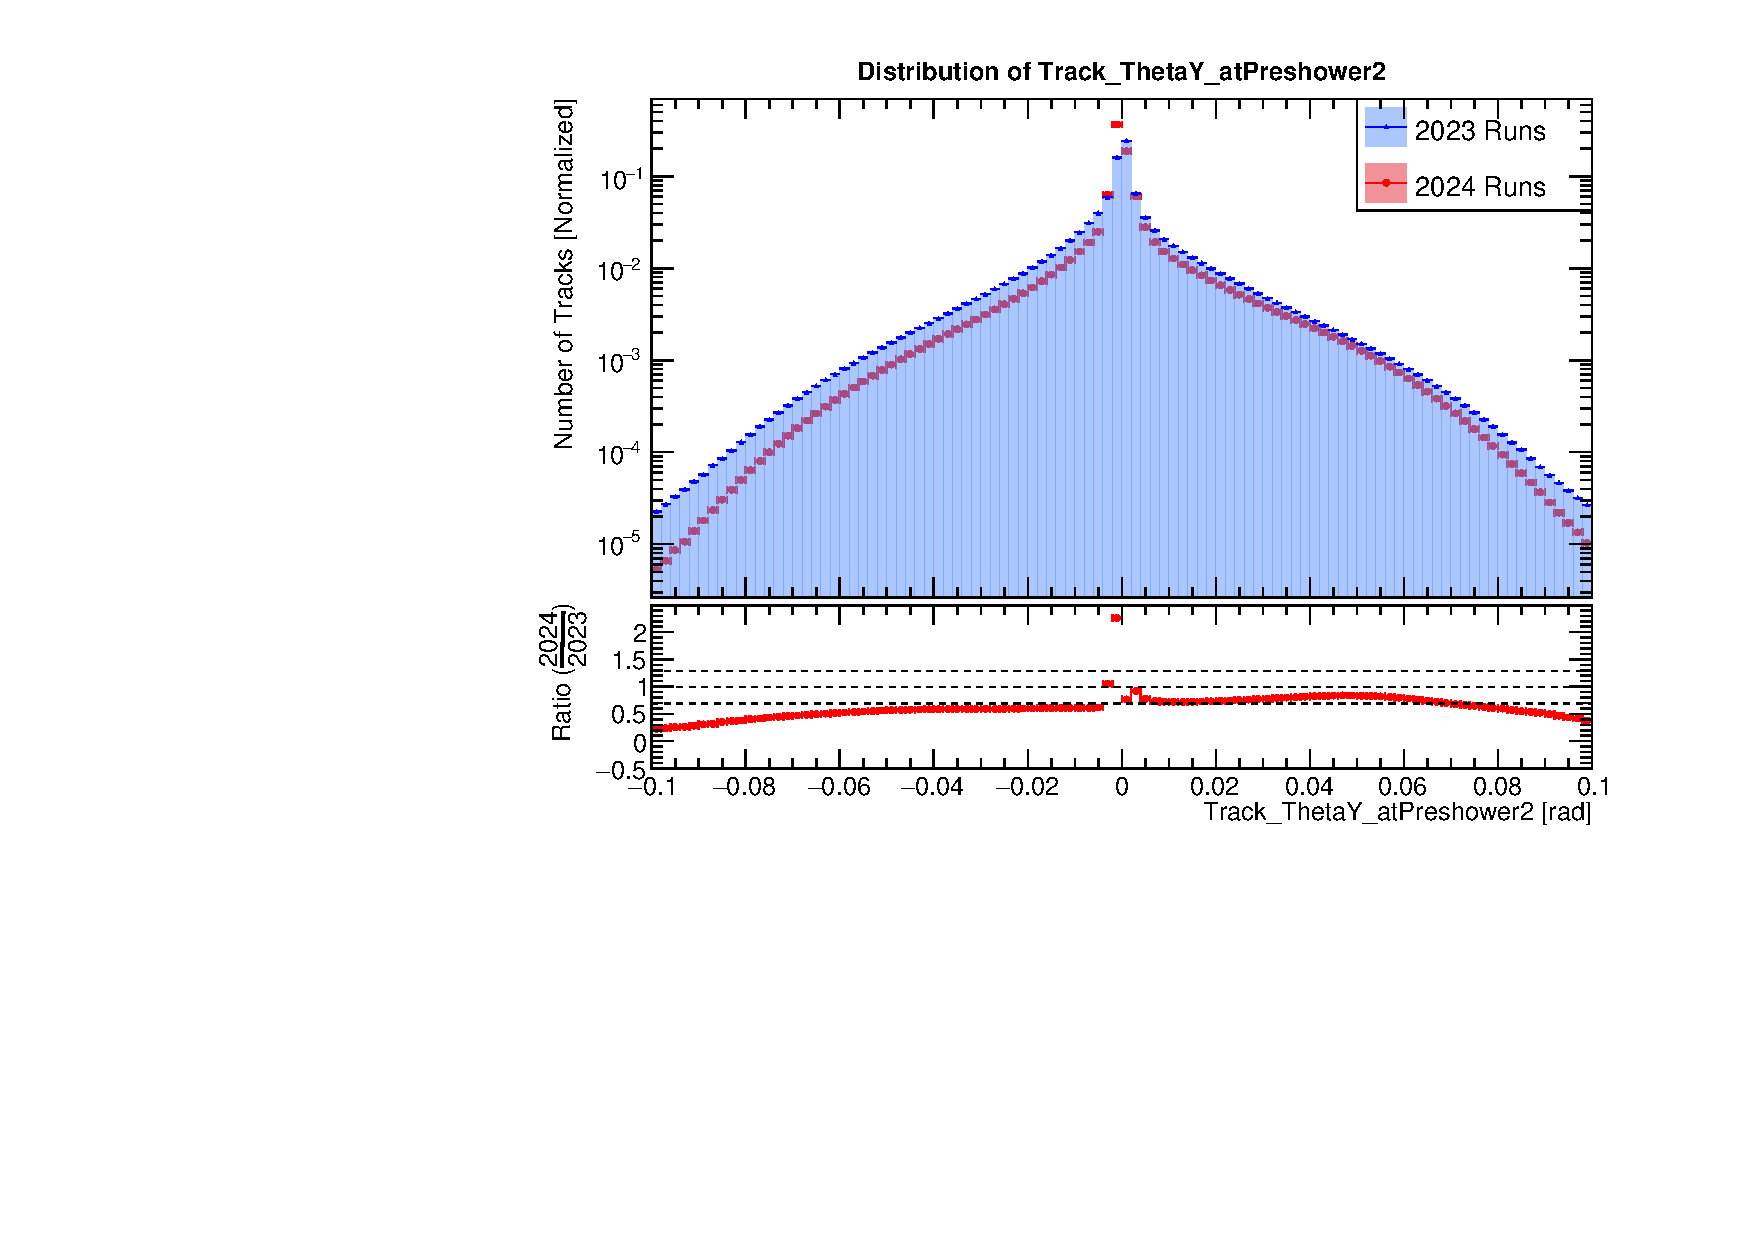
\includegraphics[width=\linewidth] {\plots/Track_ThetaY_atPreshower2.pdf}
				\caption{Track ThetaY at Preshower 2}
			\end{figure}
		\end{column}
	\end{columns}
\end{subframe}

\begin{frame}{Track Momenta at Calo}
	\begin{columns}
		\begin{column}{0.5\textwidth}
			\begin{figure}
				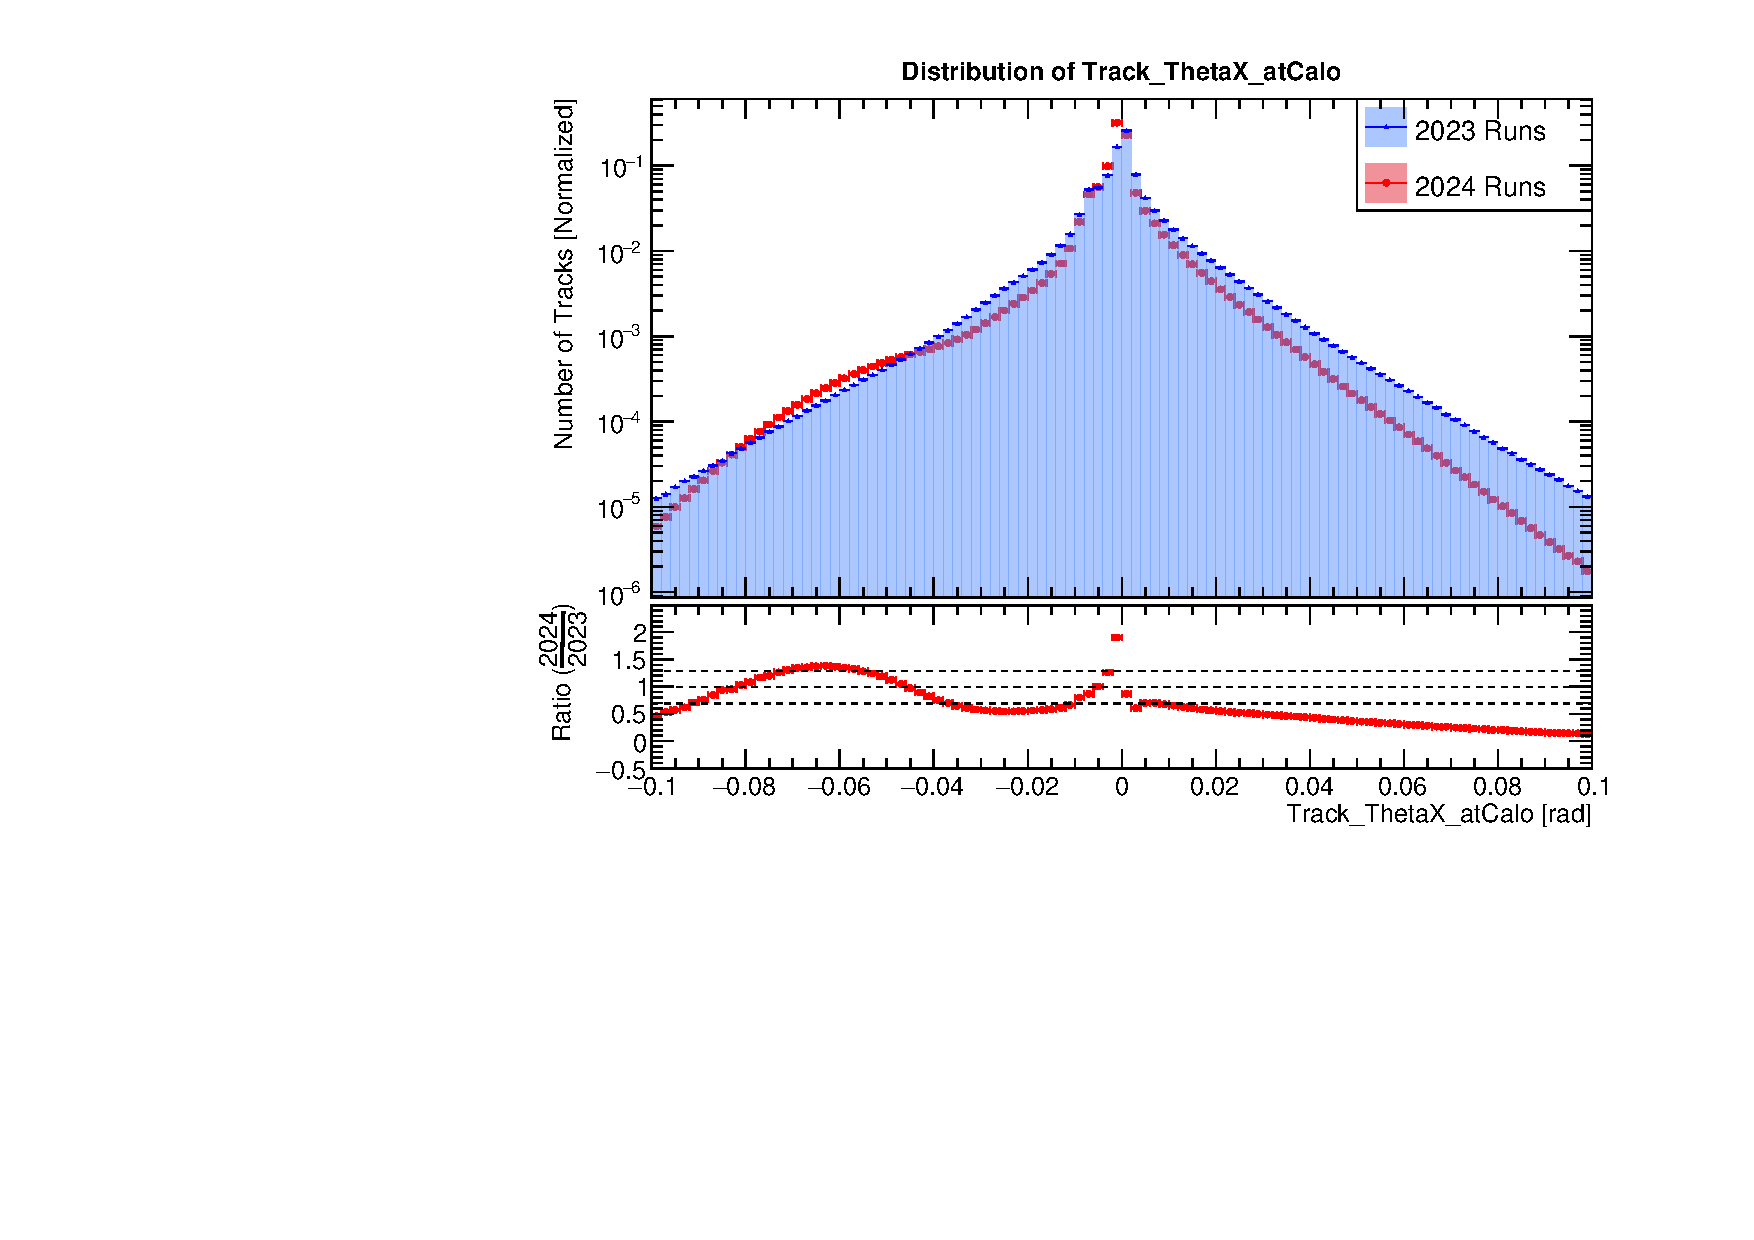
\includegraphics[width=\linewidth] {\plots/Track_ThetaX_atCalo.pdf}
				\caption{Track ThetaX at Calo}
			\end{figure}
		\end{column}
		\begin{column}{0.5\textwidth}
			\begin{figure}
				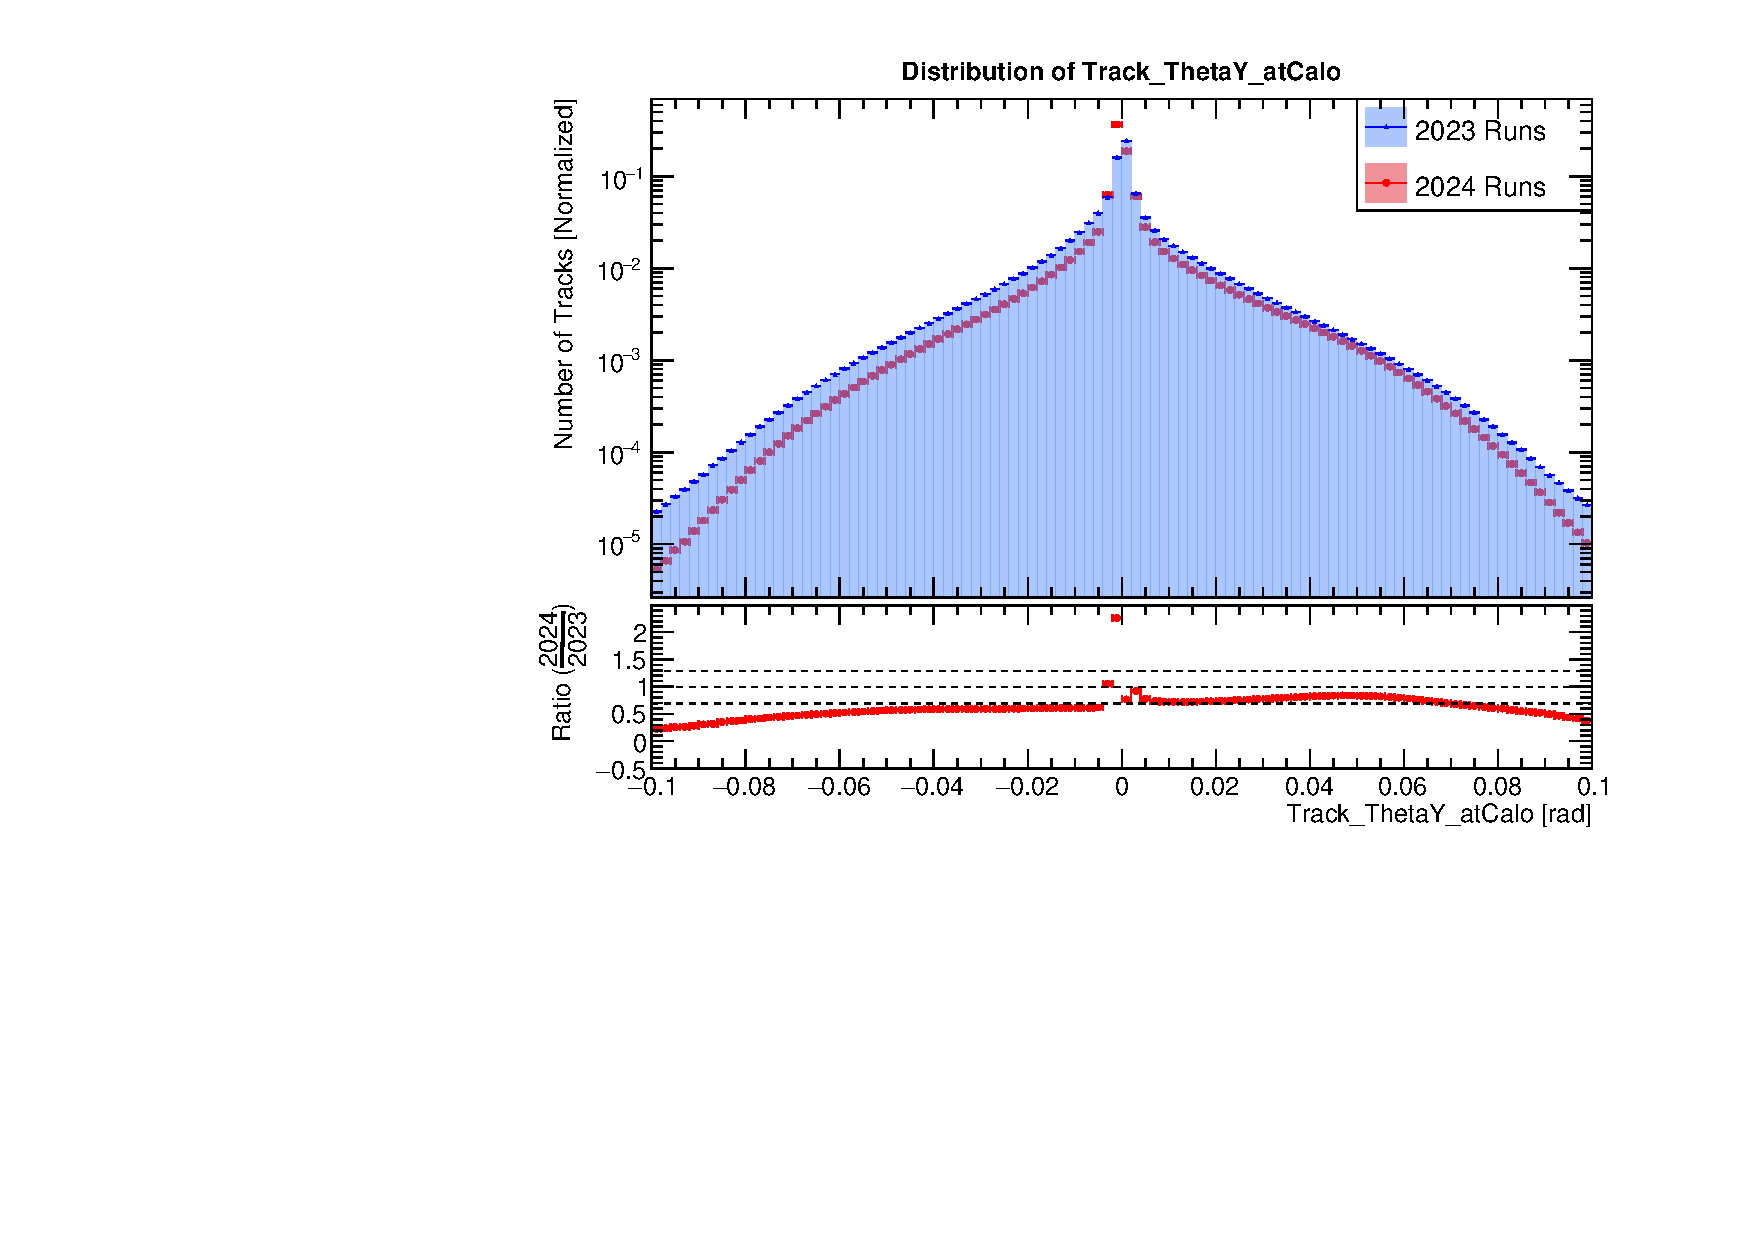
\includegraphics[width=\linewidth] {\plots/Track_ThetaY_atCalo.pdf}
				\caption{Track ThetaY at Calo}
			\end{figure}
		\end{column}
	\end{columns}
\end{frame}

\begin{frame}{Track Momenta at Tracking Station 1}
	\begin{columns}
		\begin{column}{0.5\textwidth}
			\begin{figure}
				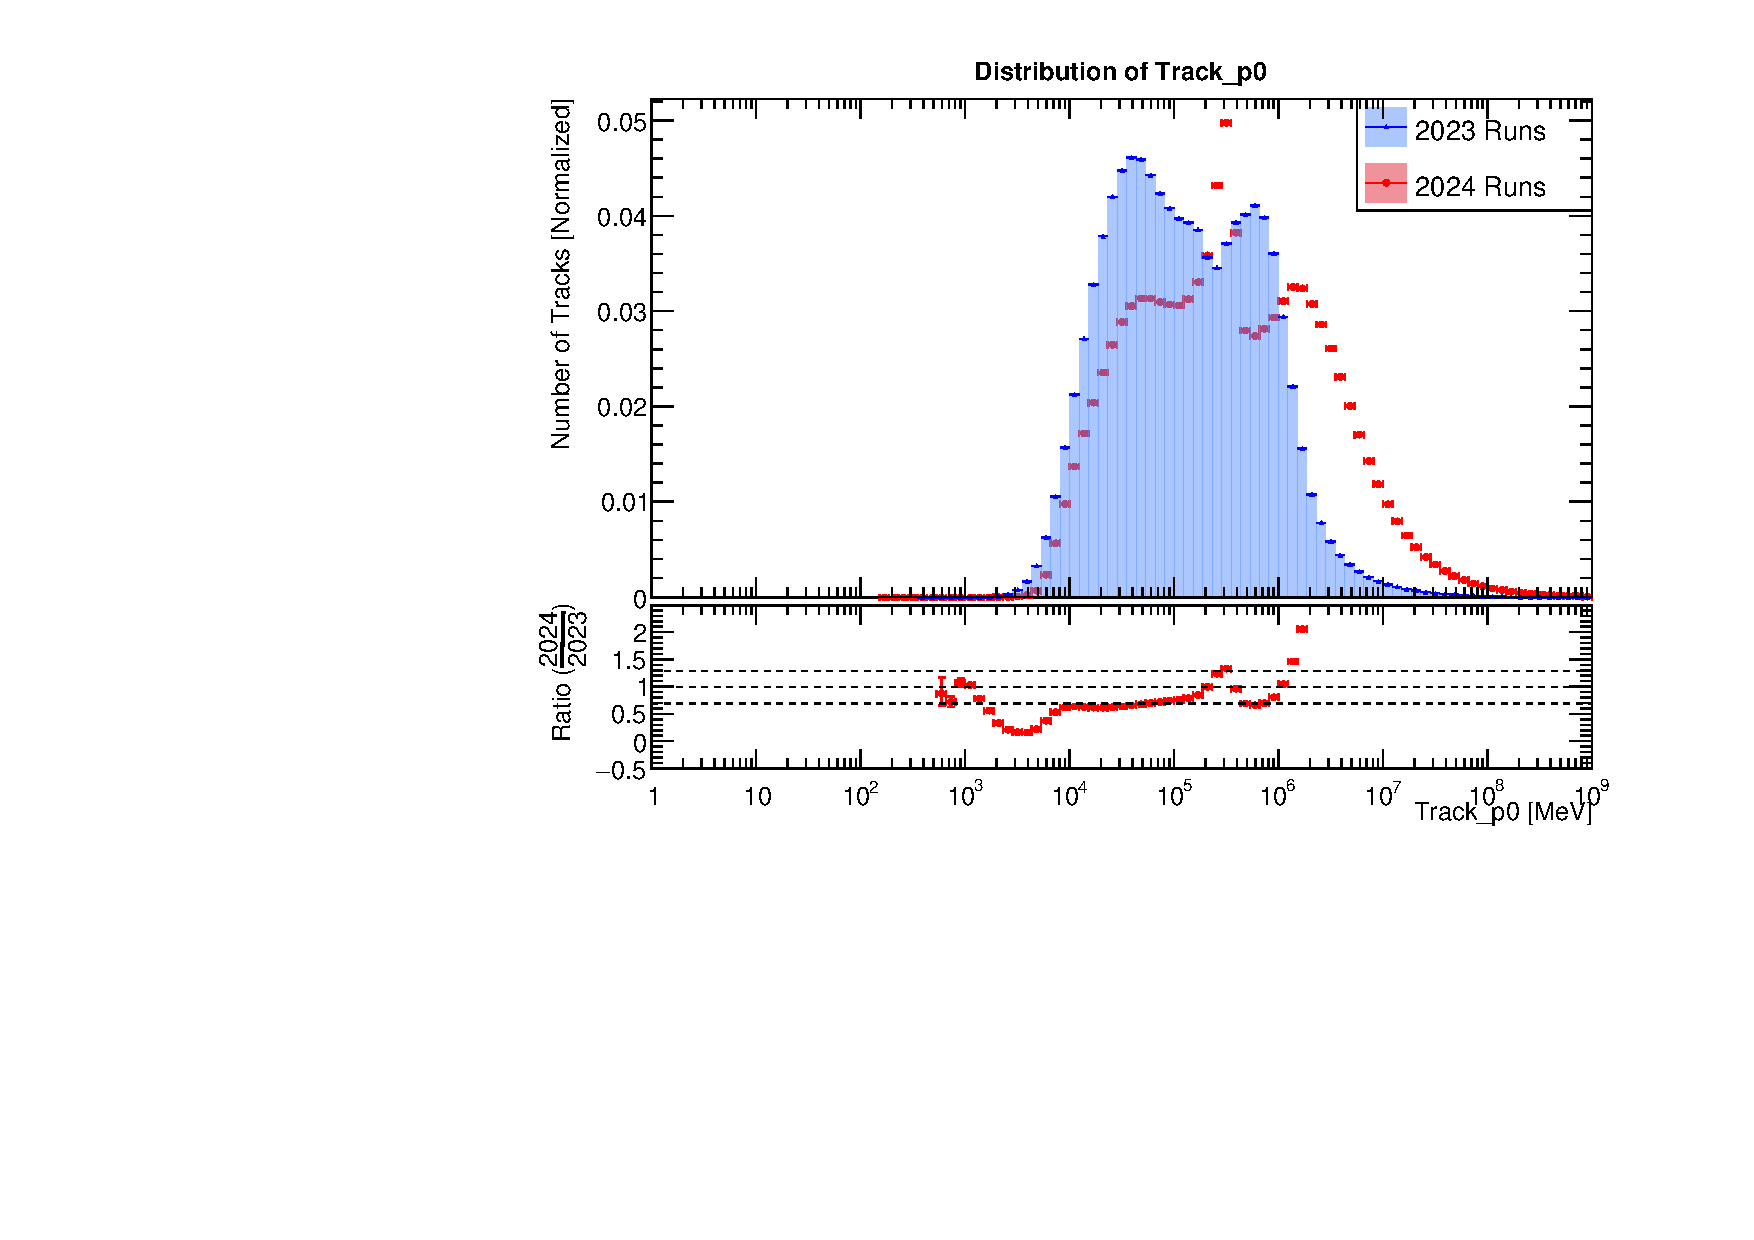
\includegraphics[width=\linewidth] {\plots/Track_p0.pdf}
				\caption{Track mometum (total) at Tracking Station 1}
			\end{figure}
		\end{column}
		\begin{column}{0.5\textwidth}
			\begin{figure}
				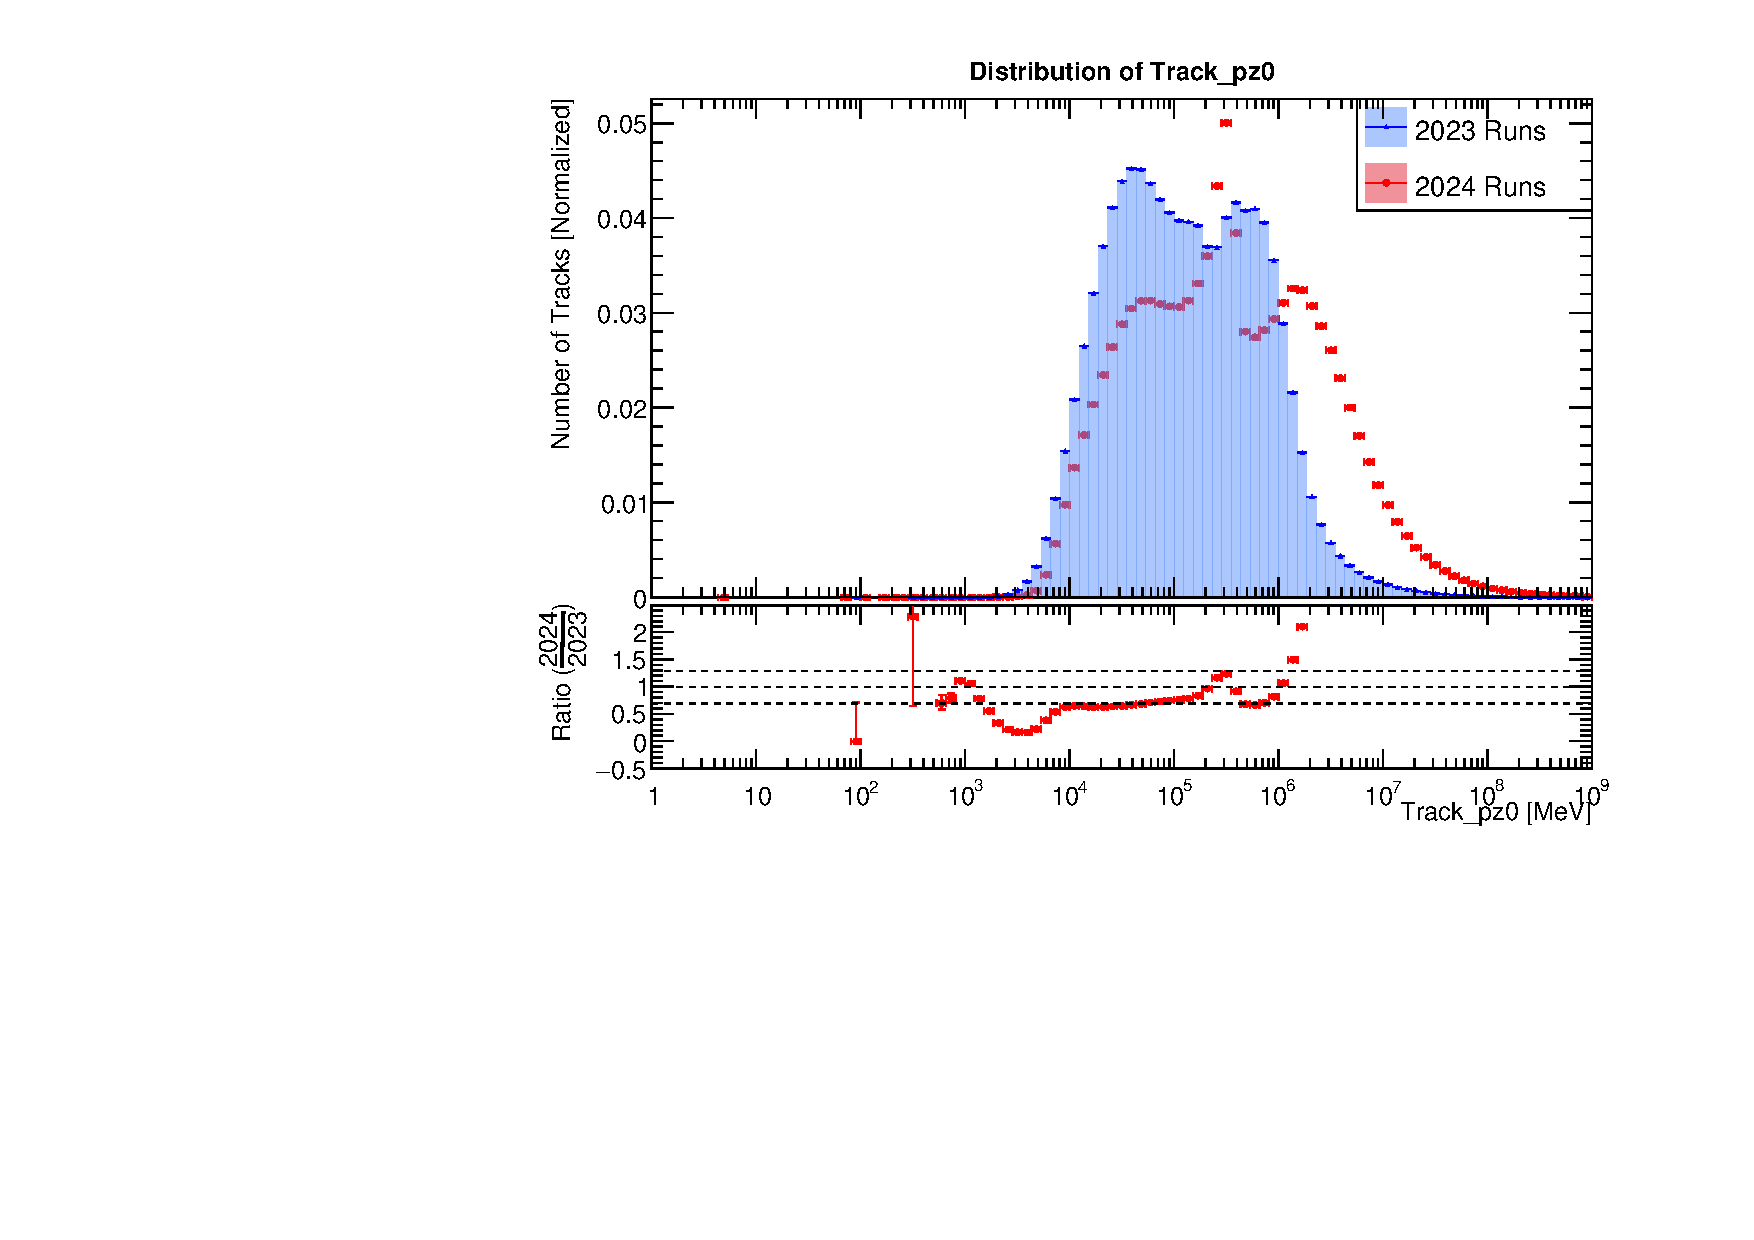
\includegraphics[width=\linewidth] {\plots/Track_pz0.pdf}
				\caption{Track momentum (pz) at Tracking Station 1}
			\end{figure}
		\end{column}
	\end{columns}
	
	\begin{itemize}
	\item We have more high momenta positively chagred muons in 2024.
	\item Background studies again showed similar features.
	\item See \href{https://indico.cern.ch/event/1350790/contributions/5686387/attachments/2836819/4957405/Introduction.pdf}{Page 15-16}
	\end{itemize}
	
\end{frame}